\documentclass[12pt, a4paper]{report}
\usepackage[utf8]{inputenc}
\usepackage[T1]{fontenc}
\usepackage[french]{babel}
\usepackage{graphicx}
\usepackage{geometry}
\geometry{hmargin=2.2cm, vmargin=2.2cm, headheight=30pt}
\usepackage{titlesec}
\usepackage{hyperref}
\hypersetup{colorlinks=true, linkcolor=black, urlcolor=blue}
\usepackage{float}
\usepackage{enumitem}
\usepackage{amsmath}
\usepackage{fancyhdr}
\usepackage{tikz}
\usepackage{eso-pic}
\usepackage{afterpage}


\pagestyle{fancy}
\fancyhf{}


\fancyhead[L]{
\includegraphics[height=1cm]{UL.png}}
\fancyhead[R]{
\includegraphics[height=1cm]{iut.png}}


\fancyfoot[C]{\raisebox{1cm}{\footnotesize\thepage}}

\renewcommand{\headrulewidth}{0pt}
\renewcommand{\footrulewidth}{0pt}


\fancypagestyle{plain}{%
  \fancyhf{}
  \fancyhead[L]{
\includegraphics[height=1cm]{UL.png}} 
  \fancyhead[R]{
\includegraphics[height=1cm]{iut.png}}  
  \fancyfoot[C]{%
  \raisebox{+1cm}{\footnotesize\thepage}%
}
  \renewcommand{\headrulewidth}{0pt}
  \renewcommand{\footrulewidth}{0pt}
}


\titleformat{\chapter}[display]
{\normalfont\huge\bfseries}{\chaptertitlename\ \thechapter}{20pt}{\Huge}
\titlespacing*{\chapter}{0pt}{-30pt}{40pt}

\titleformat{\section}
{\normalfont\Large\bfseries}{\thesection}{1em}{}
\titlespacing*{\section}{0pt}{3.5ex plus 1ex minus .2ex}{2.3ex plus .2ex}

\setlength{\parindent}{0pt}
\setlength{\parskip}{1em}

\begin{document}

\begingroup
\AddToShipoutPicture*{} 
\thispagestyle{empty}   
\begin{titlepage}
  \centering
  \vspace*{1cm}
  {\Huge\bfseries Rapport de stage\par}
  \vspace{1.5cm}
  {\LARGE Réseaux de neurones  pour la modélisation de la dynamique des véhicules\par}
  \vspace{2cm}
  {\Large Master 2 EEA : Mesure et traitement de l'information\par}
  \vspace{2cm}
  {\Large\bfseries Réalisé par :\par}
  {\Large Benabdelaziz Melissa\par}
  \vspace{1cm}
  {\Large\bfseries Encadré par :\par}
  {\Large Mr Ali Zemouche \par}
  {\Large Mr Habert Olivier\par}
  \vspace{1.5cm}
  {\Large\bfseries Année universitaire 2024/2025\par}
  \vfill
\end{titlepage}
\endgroup



\chapter*{Remerciements}
\thispagestyle{fancy}
\addcontentsline{toc}{chapter}{Remerciements}

Avant d’entamer la rédaction de ce rapport, il me semble essentiel de souligner l’assistance précieuse que j’ai reçue de la part de toutes les personnes ayant contribué, de près ou de loin, à la réalisation de ce travail.

Je tiens à exprimer ma sincère gratitude à toute l’équipe du laboratoire CRAN ainsi qu’à l’IUT de Longwy, pour m’avoir offert l’opportunité d’effectuer mon stage au sein de leurs structures cette année. Cette première expérience dans un environnement de recherche aussi enrichissant a été pour moi une véritable opportunité d’apprentissage et de développement professionnel.

Mes remerciements les plus chaleureux vont à Monsieur Ali Zemouche, mon tuteur de stage, pour son accompagnement constant, sa disponibilité, sa bienveillance et ses conseils tout au long de cette expérience. Je remercie également Huy Nguyen, doctorant au sein du laboratoire, pour son encadrement technique, sa patience et son soutien quotidien dans le suivi de mes travaux. Leur encadrement m’a permis de progresser avec rigueur et autonomie, dans un cadre de travail exigeant et stimulant.

Je souhaite aussi remercier Monsieur Boussefsaf, enseignant en intelligence artificielle, dont les cours m’ont permis d’acquérir des compétences que j’ai pu mettre en pratique concrètement durant mon stage. Son enseignement a été un véritable atout dans l’approche technique du projet qui m’a été confié.

Je tiens également à exprimer ma reconnaissance à Monsieur Olivier Habert, mon tuteur pédagogique et responsable de formation, pour son implication, son suivi attentif, et la qualité de ses enseignements qui m’ont permis de renforcer mes compétences dans mon domaine d’études.

Je souhaite également remercier mes amis et collègues stagiaires, en particulier Mohammed et Echrak, pour leur soutien, leur camaraderie et leur aide précieuse tout au long de cette expérience au laboratoire. Leur présence et leur collaboration ont rendu cette expérience encore plus enrichissante.

En guise de conclusion, je tiens à exprimer toute ma reconnaissance envers ma famille et mes proches pour leur soutien moral indéfectible et leur confiance, malgré la distance qui nous sépare

\thispagestyle{fancy}
\tableofcontents
\listoffigures
\listoftables
\thispagestyle{fancy}

\chapter*{\centering Introduction Générale } 
\addcontentsline{toc}{section}{Introduction}
\thispagestyle{fancy}
Le domaine des véhicules autonomes représente l'une des avancées technologiques les plus prometteuses et transformatrices de notre époque. La capacité des véhicules à percevoir leur environnement, à prendre des décisions et à naviguer sans intervention humaine ouvre des perspectives considérables en termes de sécurité routière, d'efficacité énergétique et de confort de déplacement. Cependant, la réalisation de systèmes de conduite autonome fiables et robustes soulève des défis complexes, notamment en ce qui concerne la modélisation précise du comportement dynamique du véhicule et la gestion des incertitudes.

La dynamique des véhicules, l'étude du mouvement des véhicules terrestres sous l'influence de forces externes et internes, est fondamentale pour la conception de systèmes de contrôle autonomes performants. Une compréhension approfondie de cette dynamique est cruciale pour prédire la trajectoire d'un véhicule, anticiper ses réactions aux commandes et assurer sa stabilité dans diverses conditions de conduite.

Dans ce contexte, mon stage a pour objectif de contribuer à l'amélioration de la modélisation de la dynamique de véhicule en utilisant des techniques d'apprentissage automatique, plus spécifiquement les réseaux de neurones. Le projet se décompose en plusieurs étapes clés : la simulation d'un véhicule virtuel (QCar) sur la plateforme Quanser Lab pour la collecte de données, l'entraînement d'un réseau de neurones récurrent pour prédire la dynamique du véhicule, l'intégration de contraintes physiques pour améliorer la robustesse du modèle, et enfin, son application dans un observateur d'état.



\chapter{Présentation générale et Contexte}
\thispagestyle{fancy}

\section{Introduction }

Ce premier chapitre a pour objectif de présenter le cadre général dans lequel s'inscrit ce projet de recherche au sein du le Centre de Recherche en Automatique de Nancy (CRAN) . Je commencerai par exposer mes missions et objectifs, structurés autour de trois pôles principaux : coordination et gestion, technique, et recherche. J'aborderai ensuite la méthodologie adoptée pour mener à bien ce projet, qui suit un enchaînement logique allant de la simulation à l'intégration du modèle.

Je présenterai ensuite le laboratoire d'accueil, , en détaillant son écosystème de recherche pluridisciplinaire et ses partenariats stratégiques.

Une introduction aux véhicules autonomes permettra de poser les bases conceptuelles et techniques nécessaires à la compréhension des enjeux, en explicitant les différents niveaux d'autonomie et le fonctionnement général de ces systèmes.

Je décrirai ensuite la plateforme expérimentale utilisée, le QCar de Quanser, en détaillant ses capteurs  et actionneurs , ainsi que les outils logiciels mobilisés .

Enfin, je terminerai par la description de l'installation et la configuration de l'environnement de développement, étape cruciale qui a précédé la phase de simulation .

Ce chapitre pose ainsi les fondations techniques et institutionnelles nécessaires à la compréhension des développements méthodologiques qui seront présentés dans les chapitres suivants.
 \newpage
\section{Missions et objectifs}

{Ce stage s'inscrit dans un programme de recherche visant à faire fonctionner un véhicule autonome, le QCar de Quanser, sans intervention humaine ,
développer des algorithmes d’estimation intelligents pour améliorer le contrôle et la sécurité des véhicules connectés et autonomes (VAC).
}

Mon objectif dans ce stage est d'entraîner un modèle intelligent capable de reproduire et de prédire la dynamique du véhicule, afin d'optimiser son contrôle et sa navigation. Le travail s'effectue dans un environnement simulé fourni par Quanser, permettant de tester et valider les algorithmes en toute sécurité.


Dès le commencement de ma mission, mes objectifs ont été définis autour de trois pôles principaux de responsabilité, en étroite coordination avec les équipes du laboratoire et mes encadrants industriels

\subsection{Pôle coordination et gestion}
Durant le stage, j'ai veillé à :
\begin{itemize}
    \item Planifier et organiser mon travail en suivant le cahier des charges et le calendrier défini, en rendant compte de l'avancement et des éventuels blocages.
    \item Gérer les ressources logicielles et documentaires nécessaires au bon déroulement des activités de recherche.
\end{itemize}

\subsection{Pôle technique}
Les objectifs techniques de mon stage visent à :
\begin{itemize}
    \item Maîtriser la plateforme expérimentale \textbf{Quanser Lab} et son interface de programmation pour la simulation et le contrôle en temps réel.
    \item Développer et exécuter des scénarios de test sur un \textbf{QCar} (véhicule miniature autonome) afin de générer des jeux de données représentatifs de ses dynamiques.
    \item Acquérir, prétraiter et structurer les données de simulation brutes (états du véhicule, entrées de contrôle) pour alimenter les phases d'apprentissage.
\end{itemize}

\subsection{Pôle recherche}

L'objectif principal de mon projet de recherche est le développement et l'implémentation d'un \textbf{observateur basé sur un modèle apprenant} pour l'estimation d'état des véhicules autonomes. Cette mission se décline en plusieurs étapes techniques :

\begin{itemize}
    \item \textbf{Modélisation Prédictive par Apprentissage} : Concevoir et entraîner un modèle de réseau de neurones capable de prédire l'état futur du véhicule (simulé). Les entrées du modèle sont l'état actuel du véhicule, son historique sur les quatre dernières pas de temps, ainsi que l'entrée de contrôle appliquée.
    \item \textbf{Intégration de Contraintes Physiques} : Améliorer la robustesse et la cohérence physique des prédictions du modèle en ajoutant une \textbf{contrainte physique} directement dans la fonction de perte lors de l'entraînement. Cette étape cruciale permet d'ancrer l'apprentissage dans les lois de la physique connue (mécanique des véhicules).
    \item \textbf{Conception de l'Observateur Hybride} : Intégrer le modèle apprenant, désormais informé par la physique (\textbf{Physics-Informed}), au sein d'une architecture d'observateur. Le but est de créer un système d'estimation fiable et performant, fusionnant la puissance de l'apprentissage machine avec la rigueur des méthodes classiques de l'automatique.
\end{itemize}

\section{Méthodologie et démarche de projet}

Ma démarche pour atteindre ces objectifs suit un enchaînement logique et expérimental :

\begin{enumerate}
    \item \textbf{Simulation et Acquisition de Données} :
    \begin{itemize}
        \item Utilisation intensive de l'environnement \textbf{Quanser Lab} pour simuler des scénarios de conduite complexes avec un ou plusieurs QCars.
        \item Conduite des véhicules en simulation pour collecter un large jeu de données contenant les séquences d'états (position, vitesse, orientation...) et les commandes associées.
    \end{itemize}
    
    \item \textbf{Entraînement du Modèle Prédictif} :
    \begin{itemize}
        \item Extraction et préparation des données enregistrées pour constituer le jeu d'entraînement.
        \item Développement et entraînement du modèle de prédiction d'état, en utilisant une fonction de perte classique puis une \textbf{fonction de perte contrainte par la physique} pour garantir la plausibilité des prédictions.
    \end{itemize}
    
    \item \textbf{Validation et intégration} :
    \begin{itemize}
        \item Validation des performances du modèle apprenant sur des scénarios de test non vus lors de l'entraînement.
        \item Intégration du modèle optimisé dans une boucle d'observation pour évaluer ses performances en temps réel et le comparer à des méthodes d'estimation traditionnelles.
    \end{itemize}
\end{enumerate}

Cette méthodologie permet de valider progressivement l'apport d'une approche \textbf{Physics-Informed Neural Network (PINN)} pour l'amélioration des capacités de perception et de décision des véhicules autonomes.
\newpage 

\section{Présentation du laboratoire CRAN à l'iut de Longwy}

Implanté aux portes de la Belgique, du Luxembourg et de l'Allemagne, l'IUT de Longwy est un établissement à dimension humaine et à forte vocation internationale depuis 1969. Au-delà de ses formations, il constitue un pôle de recherche dynamique, accueillant cinq équipes de recherche dont une antenne du CRAN (\textbf{Centre de Recherche en Automatique de Nancy}).

Fondée en 1980, le CRAN est une Unité Mixte de Recherche (UMR 7039) sous la double tutelle de l'Université de Lorraine et du CNRS. C'est une structure de grande envergure, regroupant près de 250 membres répartis sur plusieurs sites, dont environ 120 chercheurs permanents et une centaine de doctorants et post-doctorants.

Ses recherches se structurent autour de trois départements scientifiques complémentaires :

\begin{itemize}
    \item \textbf{CID} (Contrôle, Identification, Diagnostic)
    \item \textbf{MPSI} (Modélisation, Pilotage et Sûreté des Systèmes Industriels)
    \item \textbf{BioSiS} (Biologie, Signaux et Systèmes en Cancérologie et Neurosciences)
\end{itemize}

Cette organisation permet au laboratoire d'opérer à l'intersection de disciplines clés : l'automatique, le traitement du signal, l'informatique, la productique et les sciences biomédicales. Une part significative de ses travaux est aujourd'hui dédiée aux systèmes autonomes et intelligents, un domaine stratégique et résolument interdisciplinaire.

\begin{figure}[H]
    \centering
    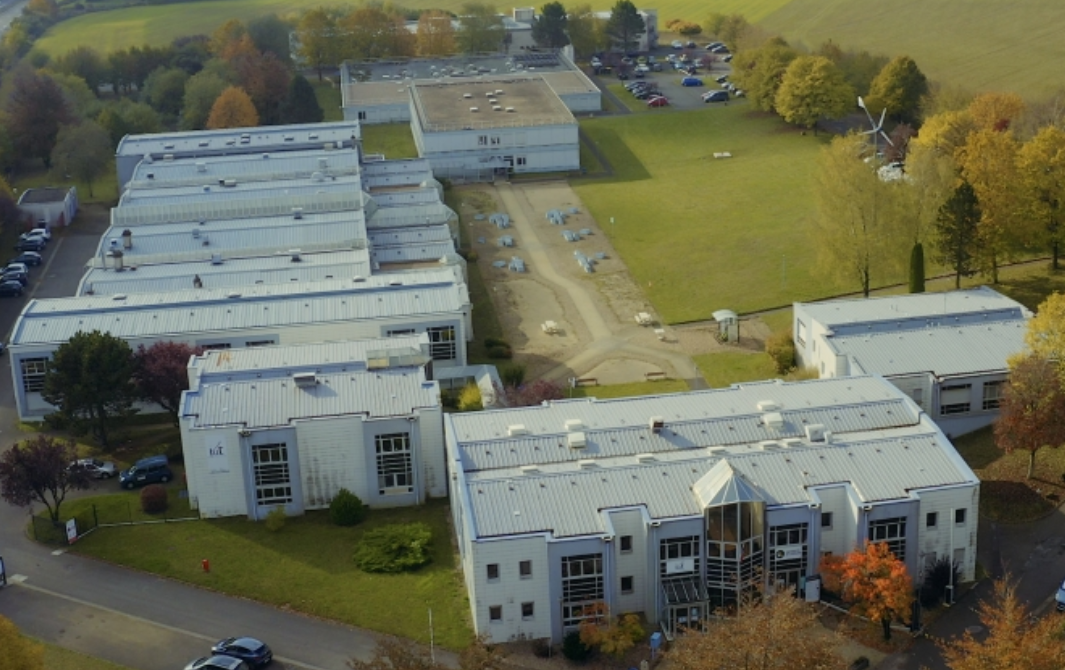
\includegraphics[width=0.7\linewidth]{lll.png}
    \caption{Site de l'IUT de Longwy }
    \label{fig:placeholder}
\end{figure}
\newpage
\subsection{Un Écosystème de recherche pluridisciplinaire et partenarial}

La force du CRAN réside dans la diversité de son équipe, qui réunit automaticiens, informaticiens, mathématiciens, biologistes et médecins. Cette pluridisciplinarité est le moteur de projets innovants, à la fois fondamentaux et appliqués.

Le laboratoire s'appuie sur un \textbf{réseau partenarial solide et diversifié}, comprenant :

\begin{itemize}
    \item \textbf{Des leaders industriels mondiaux} : Renault, Safran, EDF, ArcelorMittal, Schneider Electric, le CNES (Centre National d'Études Spatiales) et Air Liquide.
    \item \textbf{Des PME innovantes et acteurs régionaux} : PREDICT (spécialiste de la maintenance prédictive), SD Innovation (transfert technologique en santé), le CRITT Bois, ou encore Trane.
    \item \textbf{Le monde médical} : Le CHRU de Nancy et l'Institut de Cancérologie de Lorraine (ICL) pour la recherche translationnelle.
    \item \textbf{Un vaste réseau académique international} : Avec plus de 30 universités partenaires dans une vingtaine de pays (Australie, Brésil, Mexique, Allemagne, Luxembourg, Hong Kong...), le CRAN participe activement à des programmes européens et des cotutelles de thèses.
\end{itemize}

Parmi ces collaborations, le partenariat avec SEGULA Technologies. acteur majeur de l'ingénierie, se concentre sur le développement de technologies embarquées et de systèmes pour les véhicules autonomes et connectés.

\begin{figure} [H]
    \centering
    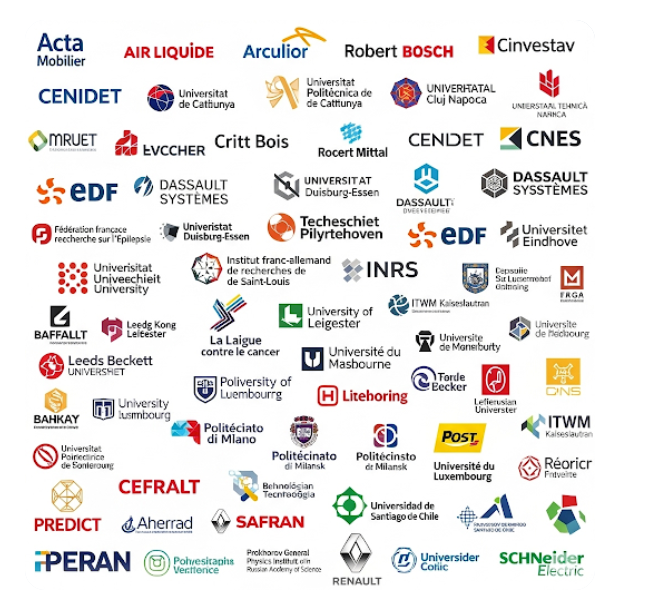
\includegraphics[width=0.6\linewidth]{kiki.png}
    \caption{collaborateurs du laboratoire Cran }
    \label{fig:placeholder}
\end{figure}

\subsection{Réalisations, projets emblématiques et partenariat stratégique}

Le CRAN est reconnu pour son excellence scientifique, avec une production annuelle de plus de 300 publications dans des revues et conférences de rang international. Ses recherches, souvent primées, ont conduit au dépôt de brevets industriels et au développement de logiciels et prototypes qui font référence.

Ses réalisations majeures couvrent un spectre très large :

\begin{itemize}
    \item \textbf{Santé} : Développement de dispositifs médicaux innovants pour le diagnostic précoce des cancers (vessie, peau) via l'imagerie hyper-spectrale et la spectroscopie.
    \item \textbf{Industrie 4.0} : Conception de systèmes de maintenance prédictive (PHM) pour l'industrie, d'algorithmes de contrôle-commande pour la sidérurgie (ArcelorMittal) ou l'aéronautique (Safran), et d'outils d'optimisation de la production pour les PMI.
    \item \textbf{Systèmes autonomes} : Recherche de pointe sur les véhicules autonomes, incluant la localisation, la planification de trajectoire et la commande robuste, testée sur des plateformes expérimentales dédiées.
\end{itemize}

La collaboration avec SEGULA Technologies incarne parfaitement la philosophie du CRAN : une recherche d'excellence au service de l'innovation industrielle. Ce partenariat stratégique, matérialisé par des thèses CIFRE, se concentre sur les défis cruciaux de la mobilité de demain. Les travaux conjoints portent sur le développement de systèmes embarqués résilients et intelligents pour les véhicules connectés et autonomes (VCA).

L'objectif est de concevoir des solutions innovantes pour renforcer la sécurité et la fiabilité des VCA, en s'attaquant à des verrous technologiques majeurs tels que :


 La détection et la mitigation des cyber-attaques visant les communications entre véhicules ou les capteurs , L'estimation fiable de variables critiques pour la conduite autonome (comme l'angle de glissement ou le risque de renversement) qui sont coûteuses ou impossibles à mesurer directement et enfin  le  développement de capteurs logiciels avancés et de cartes électroniques embarquant des algorithmes d'intelligence artificielle et d'automatique.


Cette synergie unique entre l'expertise académique de haut niveau du CRAN en modélisation, estimation et commande des systèmes complexes, et la maîtrise de SEGULA en ingénierie, intégration système et déploiement industriel, permet d'accélérer le transfert technologique. Elle positionne le CRAN comme un partenaire incontournable pour les acteurs industriels qui conçoivent les mobilités futures, en apportant des réponses concrètes et innovantes aux enjeux de sécurité et de performance.

\begin{figure}[H]
    \centering
    
\includegraphics[width=0.5\linewidth]{hhhh.png}
    \caption{Logo entreprise segula }
    \label{fig:placeholder}
\end{figure}
\newpage
\section{Introduction aux véhicules autonomes}

\subsection{Définition générale}

Un véhicule autonome est un système motorisé capable de circuler sans intervention humaine, grâce à un ensemble coordonné de capteurs, d'algorithmes de perception, de planification et de contrôle. Ces véhicules utilisent des données en temps réel pour analyser leur environnement, anticiper les comportements des autres usagers, et prendre des décisions optimales de conduite. Voici un exemple simple d'une  voiture autonome dans la Figure~\ref{fig:placeholder}, 
 \begin{figure}[H]
     \centering
     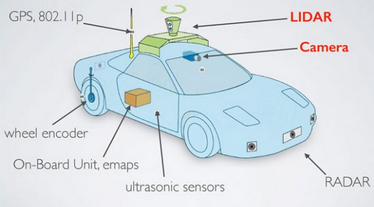
\includegraphics[width=0.5\linewidth]{va.png}
     \caption{exemple de voiture autonome et ses composants}
     \label{fig:placeholder}
 \end{figure}
\subsection{Fonctionnement global}

Le fonctionnement d'un véhicule autonome repose sur plusieurs étapes clés :

\begin{enumerate}
    \item \textbf{Perception} : collecte de données à l'aide de caméras, radars, lidars, GPS, capteurs inertiels, etc.
    \item \textbf{Compréhension} : interprétation de l'environnement (détection d'obstacles, lecture de panneaux, localisation).
    \item \textbf{Planification} : élaboration de trajectoires sécurisées et optimisées.
    \item \textbf{Contrôle} : exécution de ces trajectoires par des systèmes d'actionneurs (direction, accélération, freinage).
\end{enumerate}

\subsection{Niveaux d'autonomie}

Selon la classification SAE, il existe six niveaux :

\begin{itemize}
    \item \textbf{Niveau 0} : aucune assistance automatisée.
    \item \textbf{Niveau 1} : assistance partielle (ex : régulateur de vitesse adaptatif).
    \item \textbf{Niveau 2} : assistance combinée (direction + vitesse).
    \item \textbf{Niveau 3} : autonomie conditionnelle, l'humain peut être requis.
    \item \textbf{Niveau 4} : autonomie complète dans certaines zones ou conditions.
    \item \textbf{Niveau 5} : autonomie totale, sans intervention humaine, dans tous les environnements.
\end{itemize}

\newpage
\section{Présentation du qCar}

Le \textbf{QCar} est une plateforme mobile développée par \textbf{Quanser} pour l'enseignement et la recherche sur les véhicules autonomes. C'est un véhicule à l'échelle 1/10, pesant environ 2,7 kg, équipé d'un ensemble complet de capteurs et d'actionneurs permettant la mise en œuvre de scénarios réalistes de conduite autonome.

Le QCar est compatible avec les bibliothèques \textbf{QUARC} et \textbf{Simulink} de MATLAB, ce qui permet de développer, simuler, déployer et exécuter en temps réel des modèles de commande directement sur véhicule., 
Comme on peut le voir sur la Figure~\ref{fig:qcar_elements}le QCar est équipé de plusieurs éléments importants:  

\begin{figure}[H]
    \centering
    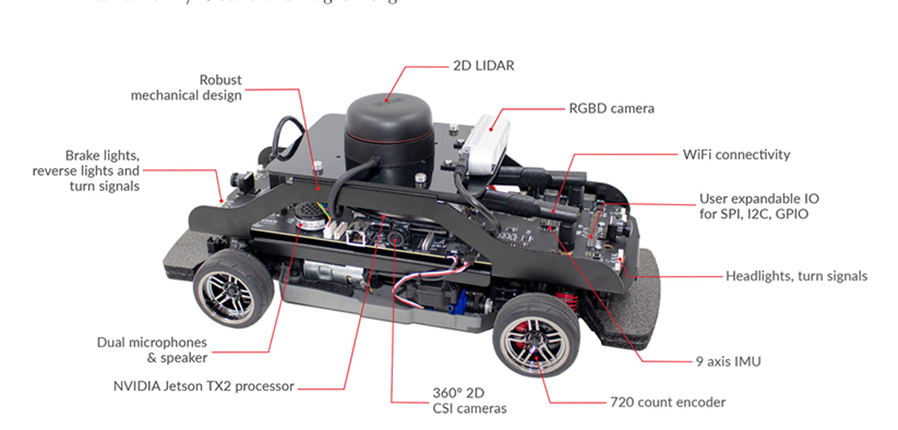
\includegraphics[width=0.7\textwidth]{qcar.png}
    \caption{Le QCar avec ses différents éléments}
    \label{fig:qcar_elements}
\end{figure}

\subsection{Lidar (Light Detection And Ranging)}

Capteur optique qui utilise un faisceau laser pour mesurer la distance entre le véhicule et les objets environnants, en balayant l'environnement en 2D ou 3D.

Son rôle est de créer une carte en temps réel des obstacles et de l'environnement, indispensable pour la navigation autonome et l'évitement d'obstacles.

En ce qui concerne notre projet il est utile pour la détection des obstacles fixes ou mobiles et intégration dans la planification de trajectoire.


\begin{figure}[H]
    \centering
    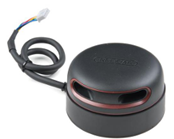
\includegraphics[width=0.2\textwidth]{lidar.png}
    % REMPLACER LE CHEMIN ET LE NOM DU FICHIER
    \caption{LIDAR du QCar}
    \label{fig:qcar_lidar}
\end{figure}

\subsection{Caméras RGB et RGBD}

Caméras classiques (RGB) capturant des images en couleur et caméras RGBD capturant en plus la profondeur pour chaque pixel.

Son rôle est de fournir des images pour la vision par ordinateur (détection de lignes, panneaux, objets) et des données de profondeur pour mesurer les distances.

La caméra est utile dans notre projet pour le suivi de voie (lane following), reconnaissance visuelle, localisation visuelle.


\begin{figure}[H]
    \centering
    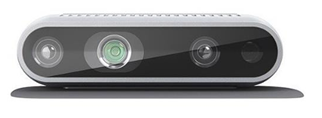
\includegraphics[width=0.5\linewidth]{camera.png}
    \caption{Caméras du QCar}
    \label{fig:qcar_cameras}
\end{figure}

\subsection{Encodeurs de roues}

 Capteurs mesurant le nombre de rotations effectuées par les roues , il sert à  calculer la distance parcourue et la vitesse des roues , de plus il  mesure en précision  la vitesse longitudinale .

\subsection{Moteurs électriques}

 Actionneurs assurant la propulsion du QCar , son rôle est de  convertir les commandes de vitesse en mouvement réel , il peut aussi  contrôler  l'accélération et le  freinage.

\subsection{Servo-moteur de direction}
 Moteur spécifique pour orienter les roues avant , son rôle est d'appliquer l'angle de braquage commandé par l'algorithme et de  suivre  la trajectoire de l'appareil .

\subsection{Ordinateur embarqué et connectivité Wi-Fi}

 Mini PC intégré dans le QCar, relié à un routeur Wi-Fi double bande (2,4 GHz et 5 GHz) , son rôle est de faire tourner les programmes en temps réel, communiquer avec l'ordinateur de développement , exécuter  des scripts Python et Simulink et enfin  transfert de données.
 
\subsection{Batterie et système d'alimentation}

 Batterie rechargeable offrant environ 2 heures d'autonomie , il sert à  alimenter le QCar et ses capteurs. Gestion de l'autonomie pendant les essais prolongés.

 \subsection{IMU (Inertial Measurement Unit)}

Module regroupant un gyroscope, un accéléromètre et parfois un magnétomètre pour mesurer les accélérations et vitesses angulaires.
son rôle est  d'estimer l'orientation et les mouvements du véhicule.
dans notre projet il sert à compléter ou corriger la position estimée par le modèle .

\begin{figure}[H]
    \centering
    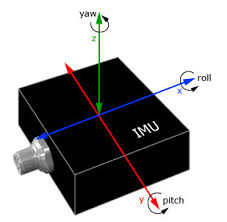
\includegraphics[width=0.5\linewidth]{unit.jpg}
    \caption{IMU}
    \label{fig:placeholder}
\end{figure}
\newpage
\section{Outils utilisés}

\subsection{Quanser Interactive Labs}

C'est l'environnement de simulation développé par Quanser pour reproduire des scénarios réalistes de circulation et de navigation. Il permet de créer des mondes virtuels avec des routes, intersections, feux de signalisation, et autres véhicules. Les interactions sont gérées en temps réel, ce qui permet de tester des algorithmes comme le suivi de trajectoire, l'évitement d'obstacles ou la navigation autonome, sans risques matériels.
\begin{figure}[H]
    \centering
    \begin{minipage}{0.45\textwidth}
        \centering
        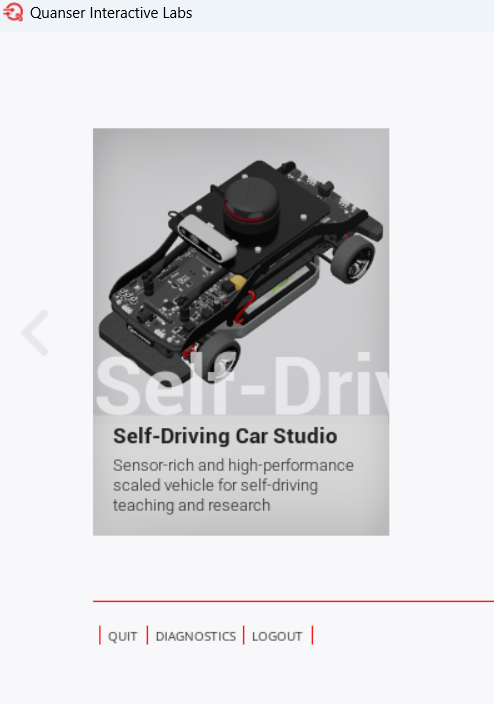
\includegraphics[width=0.5\linewidth]{image.png}
    \end{minipage}
    \hfill
    \begin{minipage}{0.45\textwidth}
        \centering
        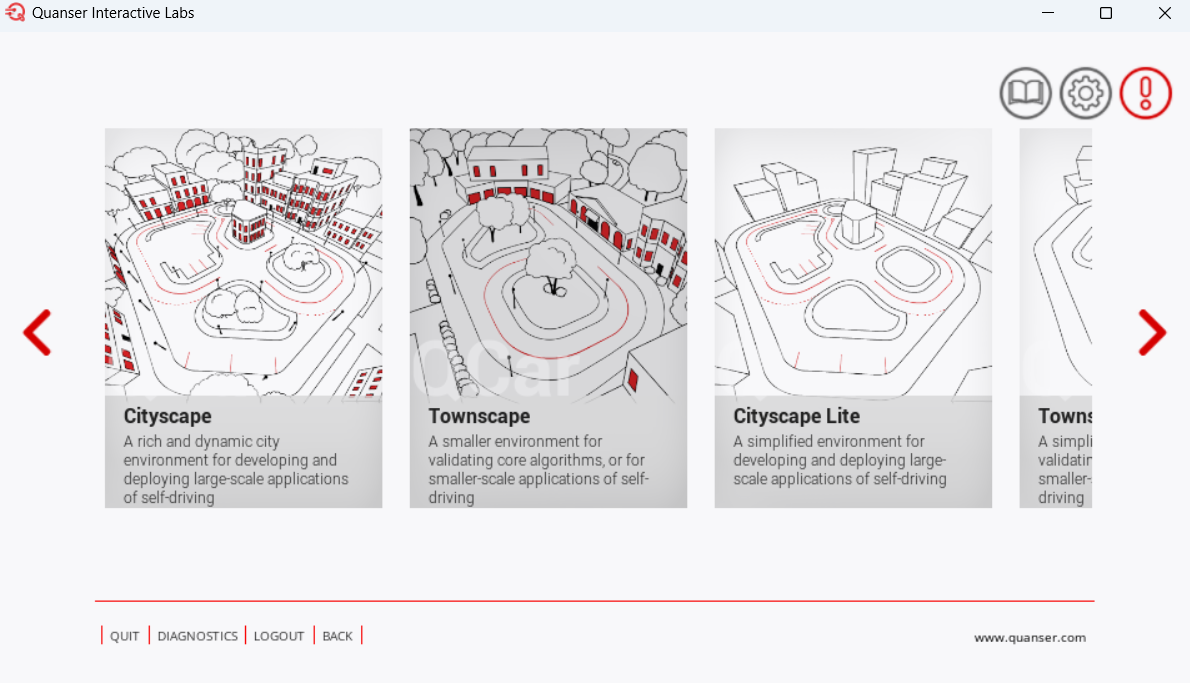
\includegraphics[width=\linewidth]{3.png}
    \end{minipage}
    \caption{Interface Quanser Interactive Labs}
    \label{fig:qcar_interface}
\end{figure}

\subsection{Quanser SDK}

Le SDK (Software Development Kit) de Quanser fournit les bibliothèques et fonctions nécessaires pour interagir avec le QCar en simulation ou en réel. Il offre un accès direct aux capteurs et actionneurs, ce qui permet de lire des données comme la vitesse, l'angle de direction, et de contrôler le véhicule via des commandes programmées. Le SDK est compatible avec plusieurs langages, dont Python et C++.

\begin{figure}[H]
    \centering
    
    
\includegraphics[width=0.5\textwidth]{qun.png}
    \caption{Logo Quanser SDK}
    \label{fig:quanser_sdk}
\end{figure}
\newpage

\subsection{Visual Studio Code}

VS Code est l'éditeur de code choisi pour ce projet, car il offre une interface légère mais puissante. Il intègre des fonctionnalités comme l'autocomplétion, le débogage, la gestion des environnements virtuels Python, et la connexion à Docker. Son extensibilité via des plugins permet d'ajouter rapidement des outils adaptés aux besoins du développement scientifique.


\begin{figure}[H]
    \centering
    
\includegraphics[width=0.2 \linewidth]{vs.png}
    \caption{Logo VS Code }
    \label{fig:placeholder}
\end{figure}
\subsection{Docker}


Docker permet de créer un environnement de développement isolé et reproductible. En encapsulant toutes les dépendances logicielles et bibliothèques nécessaires au projet, il garantit que le code pourra fonctionner de la même manière sur différents ordinateurs. Cela évite les conflits de versions et facilite le déploiement.
\begin{figure} [H]
    \centering
    
\includegraphics[width=0.3\linewidth]{ee.png}
    \caption{Logo Docker}
    \label{fig:placeholder}
\end{figure}
\newpage  

\section{Installation et configuration de l'environnement Quanser}

\subsection{Préparation}

\begin{enumerate}
    \item On a téléchargé et installé Quanser Interactive Labs via la documentation officielle , en suivant le lien : https://qlabs.quanserdocs.com/en/latest/Get%20Started.html#python-package-update
    
    
   
    \begin{figure}[H]
        \centering
        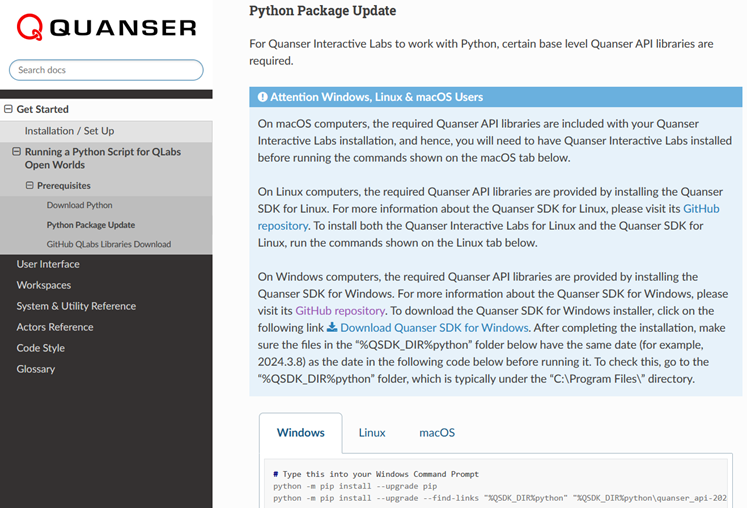
\includegraphics[width=0.5\textwidth]{4.png}
        \caption{présentation du site Qaunser}
        \label{fig:quanser_logo}
    \end{figure}
    
     \end{enumerate}

\begin{enumerate}
    \setcounter{enumi}{1} % Continue à partir de 2
    \item Par la suite on crée  un environnement virtuel Python dédié au projet.  % Devient le numéro 2

    \begin{figure}[H]
    \centering
    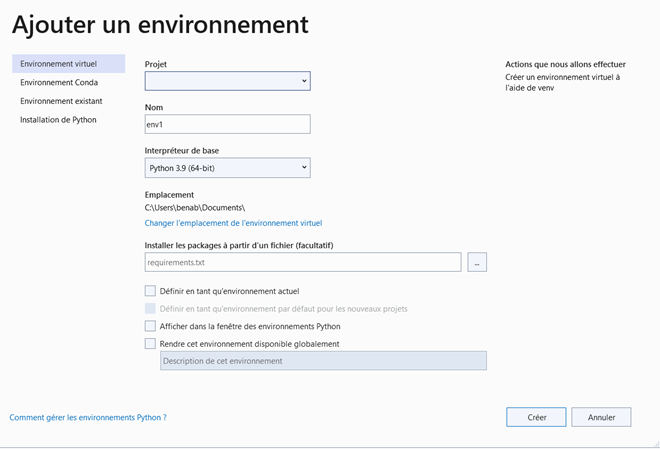
\includegraphics[width=0.8\textwidth]{image2.png}
    \caption{Création de l'environnement Python}
    \label{fig:python_env}
\end{figure} 
\newpage

    \item Enfin , on passe  à l'istallation du   SDK Quanser et des bibliothèques nécessaires avec pip.  % Devient le numéro 3
\end{enumerate}

\subsection{Configuration du simulateur}

\begin{itemize}
    \item On télechrage  le script install.py fourni par Quanser, on l'exécute pour installer les ressources.
    
    \begin{figure}[H]
        \centering
       
        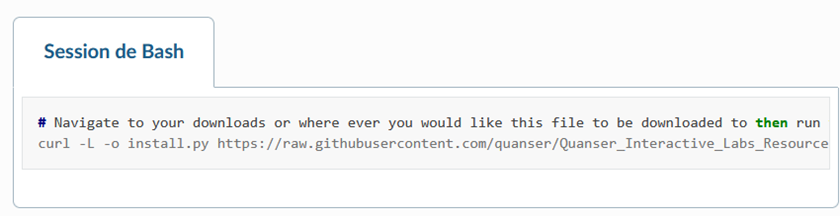
\includegraphics[width=0.5\textwidth]{pip.png}
        \caption{Exécution du script install.py}
        \label{fig:install_script}
    \end{figure}
   
    \item On lance le fichier setup.bat situé dans \textbf{Research Resources.zip} afin de configurer les dossiers et fichiers de simulation.
    \item on charge  un tutoriel de QCar2 pour vérifier le bon fonctionnement.
 
    \begin{figure}[H]
        \centering
        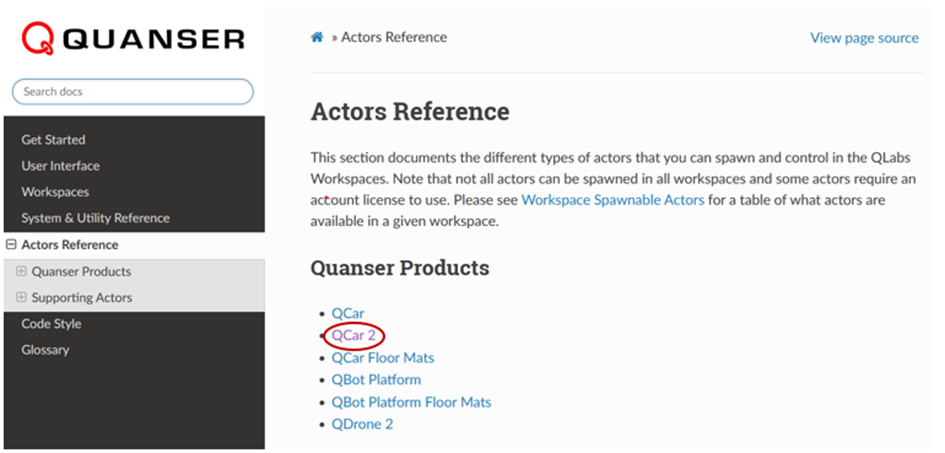
\includegraphics[width=0.8\textwidth]{ll.png}
        \caption{Interface de Quanser Interactive Labs}
        \label{fig:qlabs_interface}
    \end{figure}
  
    
\end{itemize}
\newpage

\subsection{Vérifications}

\begin{itemize}
    \item On Démarre  la scène \textit{Cityscape Lite}, comme le montre la figure~\ref{fig:qcar2_tutorial}.
    \begin{figure}[H]
        \centering
        % REMPLACER LE CHEMIN ET LE NOM DU FICHIER
        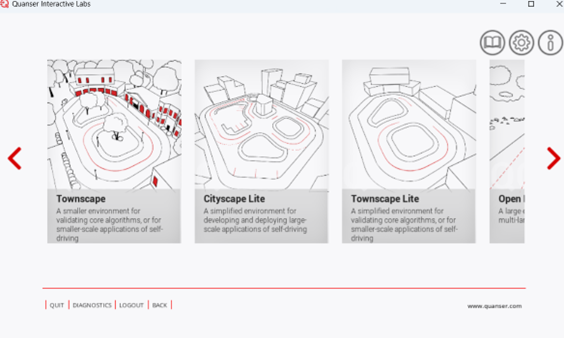
\includegraphics[width=0.8\textwidth]{kk.png}
        \caption{cityscape Lite  Quanser Interactive Labs}
        \label{fig:qcar2_tutorial}
    \end{figure}
    
  
   
    \item On s'assure  que les caméras et capteurs du QCar sont actifs.
    \item On lance  un script de test (par exemple un scénario leader/follower) pour valider la communication avec le simulateur.
    \item Une fois que l'application est en marche on obtient ça :
    
    
    \begin{figure}[H]
        \centering
         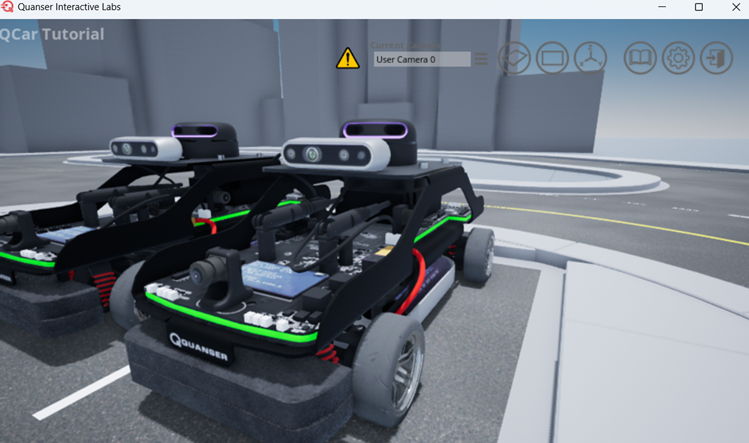
\includegraphics[width=0.5\linewidth]{encours.png}
        \caption{Vue de la simulation en cours}
        \label{fig:simulation_view}
    \end{figure}
Afin de mieux visualiser l’environnement de simulation, il est possible d’examiner l’interface de contrôle. Celle-ci permet de configurer les paramètres du véhicule, de lancer les scénarios et de suivre en temps réel l’évolution des variables dynamiques. Une vue plus détaillée est présentée sur la figure \ref{fig:control_interface}.
   
    \begin{figure}[H]
        \centering
       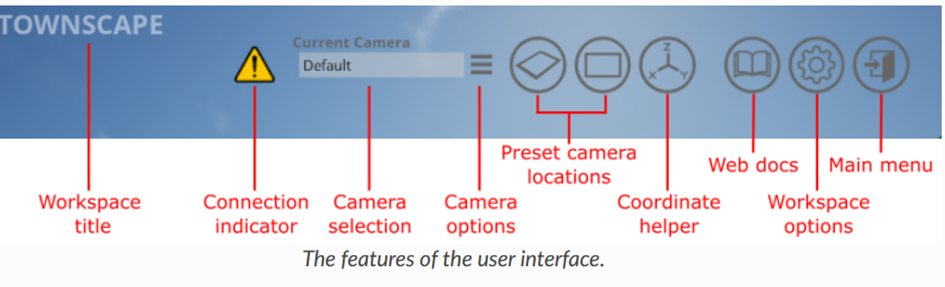
\includegraphics[width=0.8\linewidth]{cc.png}
        \caption{Interface de contrôle de la simulation}
        \label{fig:control_interface}
    \end{figure}
   
    \item \textbf{Connection Indicator} : Indicateur de connexion
    
    Le symbole d'exclamation jaune apparaîtra lorsqu'il n'y a pas d'externe actif connexion. Ces connexions peuvent être un modèle en temps réel pré-compilé, un modèle en temps réel complété par l'utilisateur, ou un script utilisant les API QLabs.
    
    \item \textbf{Sélection de la caméra}
    
    Dialogue répertoriant toutes les caméras actives. Ce dialogue affiche la liste de toutes les caméras actuellement actives dans la scène. Tout acteur intégrant des caméras, comme ceux utilisant QCar ou QBot Platform, y ajoute automatiquement ses caméras lorsqu'il est généré dans le monde. Les caméras utilisateur peuvent également être ajoutées manuellement.
    
    \item \textbf{Options pour les caméras}
    
    Accéder aux réglages de la caméra. Ceux-ci incluent les paramètres standard de la caméra utilisateur.
    
    \item \textbf{Emplacements de caméras prédéfinies}
    
    Dans certains mondes ouverts, des points d'intérêt sont définis à l'avance. La caméra par défaut sera alors automatiquement placée à ces emplacements.
    
    \item \textbf{Aide à la coordination}
    
    Utilisé pour aider à déterminer les sites de coordination dans le monde.
    
    
 \item \textbf{Options de l'espace de travail}
    
    Visualisez  l'adresse IP PC et (en mode avancé) affichez tous les paramètres graphiques
 \item     \textbf{ Onglet de diagnostic}
 Sur le côté gauche de l'écran, en cliquant sur l'onglet rouge ouvrira les diagnostics panneau qui peut fournir des informations précieuses sur les raisons pour lesquelles un acteur ne fraye pas lorsque l'on s'y attendait, les questions d'octroi de licences et les informations sur la connectivité
 \end{itemize}

\newpage
\section{Installation et configuration de l'environnement de développement}

\subsection{Structure du projet}
Une fois Visual Studio Code installé, nous créons un dossier dédié où seront placés tous les fichiers de code nécessaires pour exécuter les simulations avec une ou plusieurs voitures,nous avons utilisé python comme language de programmation  .


\subsection{Exécution des scripts}
Pour exécuter les scripts, nous utilisons le terminal PowerShell et entrons les commandes suivantes selon le script voulu :


\subsection{Script 1 : TEST (Simulation leader-follower)}

\textbf{Objectif :} \\
Mettre en place un environnement virtuel avec deux véhicules QCar2 : un leader et un follower.

\textbf{Étapes et fonctionnalités principales :}

\begin{enumerate}
    \item \textbf{Connexion à QLabs :}
    \begin{itemize}
        \item Initialisation de la communication avec QLabs
        \item Suppression de tous les objets précédemment créés
    \end{itemize}

    \begin{figure}[H]
        \centering
        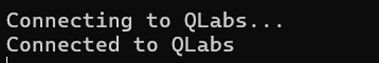
\includegraphics[width=0.5\linewidth]{coo.png}
        \caption{connection de Qlabs}
        \label{fig:placeholder}
    \end{figure}

    \item \textbf{Création de l'environnement :}
    \begin{itemize}
        \item Sol (QLabsQCarFlooring)
        \item Murs (QLabsWalls) 
        \item Passage piéton (QLabsCrosswalk)
        \item Ligne directrice (spline) pour guider le leader
    \end{itemize}
 
La mise en place de l’environnement de simulation constitue une étape essentielle pour garantir la cohérence des expériences. Avant que les véhicules puissent évoluer, il est nécessaire de définir un environnement ainsi que les différents scénarios utilisés par le modèle. La figure \ref{fig:placeholder} illustre l’aboutissement de ce processus de création.

\begin{figure} [H]
    \centering
    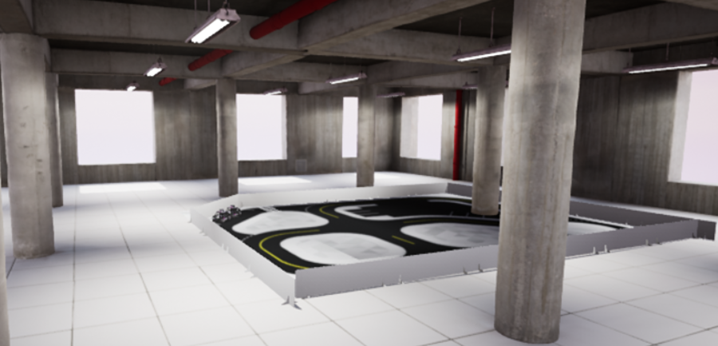
\includegraphics[width=0.5\linewidth]{gg.png}
    \caption{ création de l'environement }
    \label{fig:placeholder}
\end{figure}
    \item \textbf{positionnement  des voitures :}
    \begin{itemize}
        \item  Le spawn des voitures est réalisé en positionnant le véhicule leader et le véhicule follower avec une orientation spécifique, comme illustré à la figure \ref{fig:placeholder}
    \end{itemize}
    \begin{figure}[H]
        \centering
        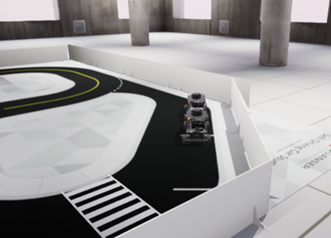
\includegraphics[width=0.5\linewidth]{ii.png}
        \caption{image du leader et du follower }
        \label{fig:placeholder}
    \end{figure}

    \item \textbf{Exécution du modèle temps réel pour le leader :}
    \begin{itemize}
        \item Chargement d'un modèle pour contrôler le mouvement du leader
    \end{itemize}

    \item \textbf{Lancement de la logique de suivi (Follower) :}
    \begin{itemize}
        \item Le follower suit dynamiquement la trajectoire du leader en temps réel
    \end{itemize}

    \item \textbf{Nettoyage :}
    \begin{itemize}
        \item Fermeture propre de la connexion à QLabs
    \end{itemize}
\end{enumerate}
\textbf{Résumé :} \\
Ce script prépare un scénario de suivi de véhicule dans un environnement simulé où un leader est contrôlé par un modèle et un follower suit dynamiquement sa trajectoire.
\newpage
\subsection{Script de contrôle du véhicule}

\textbf{Objectif :} \\
Développer un script permettant de contrôler à la fois la vitesse et la direction du QCar autonome. Pour la direction, un contrôleur Stanley est utilisé afin d'assurer le suivi précis de la trajectoire dans un scénario de navigation basé sur une carte.

\begin{figure}[h!]
    \centering
    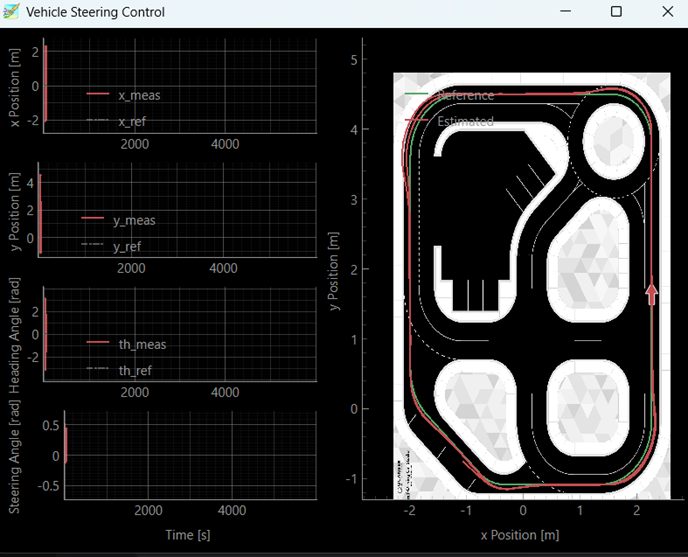
\includegraphics[width=0.8\textwidth]{mm.png}
    \caption{Interface de contrôle du véhicule dans l'environnement de simulation}
    \label{fig:vehicle_control}
\end{figure}

\textbf{Fonctionnalités principales :}

\begin{enumerate}
    \item \textbf{Paramètres d'expérience :}
    \begin{itemize}
        \item Durée (tf)
        \item Fréquence d'échantillonnage (controllerUpdateRate)
        \item Consigne de vitesse (v\_ref)
        \item Gains de contrôle (Kp, Ki pour la vitesse ; K\_stanley pour la direction)
    \end{itemize}

    \item \textbf{Chargement de la carte et génération de trajectoire :}
    \begin{itemize}
        \item Génération d'un chemin à suivre via nodeSequence
    \end{itemize}

    \item \textbf{Contrôleurs définis en classes :}
    \begin{itemize}
        \item SpeedController : régulation de vitesse via PID simplifié
        \item SteeringController : suivi de chemin via algorithme Stanley (calcul de l'angle de braquage basé sur la déviation et l'orientation)
    \end{itemize}
\newpage
    \item \textbf{Boucle de contrôle (controlLoop) :}
    \begin{itemize}
        \item Lecture des capteurs du QCar (gyroscope, tachymètre, GPS)
        \item Mise à jour de l'estimation de position via filtre EKF
        \item Calcul des signaux de commande (u pour accélération, delta pour direction)
        \item Envoi des commandes au QCar
    \end{itemize}

    \item \textbf{Visualisation avec MultiScope :}
    \begin{itemize}
        \item Affichage temps réel de la vitesse, erreur, braquage, position sur carte
    \end{itemize}
\end{enumerate}

\textbf{Résumé :} \\
Ce script implémente un contrôle autonome complet pour un véhicule suivant un chemin prédéfini sur une carte, avec contrôle de la vitesse et de la trajectoire, et interface de visualisation temps réel.
\begin{figure}[h!]
    \centering
    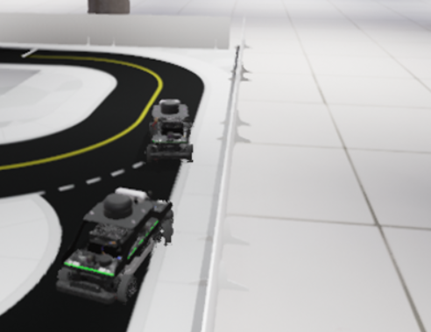
\includegraphics[width=0.6\textwidth]{simu.png}
    \caption{QCar en action dans l'environnement de simulation}
    \label{fig:qcar_simulation}
\end{figure} 

\section{Collecte de Données}

\subsection{Processus de collecte après simulation}

Après avoir configuré et exécuté les différentes simulations avec QLabs et le QCar virtuel , nous avons procédé à la collecte systématique des données selon le protocole suivant :
\begin{enumerate}

    \item \textbf{Définition du scénario} : Comme nous l'avons cité précédemment ,nous avons paramétré des sessions de 30 minutes pour chaque type de scénario. Trois catégories ont été retenues : circuit fermé, conduite urbaine et manœuvres spécifiques. Chaque essai a été configuré avec des conditions initiales précises.
    \item {Boucle d'acquisition} : À chaque pas de temps de 10 ms (100 Hz), nous acquisitions les commandes et les données capteurs. Les entrées incluaient l'accélération et l'angle de braquage. Les sorties comprenaient la position, la vitesse, l'orientation et les données IMU.
    \item \textbf {Post-traitement} : Les données brutes ont été vérifiées pour éliminer les valeurs aberrantes. Nous avons normalisé les variables pour l'apprentissage automatique. Les données ont finalement été structurées en séquences temporelles pour l'entraînement.
\end{enumerate}
Le table~\ref{tab:donnee} représente un exemple d'un extrait des données collectées.

\begin{table}[h!]
\centering
\caption{Extrait représentatif des données collectées}
\label{tab:donnee}
\begin{tabular}{|c|c|c|c|c|c|}
\hline
Temps (s) & Accélération & Direction (rad) & X (m) & Y (m) & Vitesse (m/s) \\
\hline
0.00 & 0.10 & 0.00  & 0.00 & 0.00  & 0.00 \\
0.01 & 0.15 & 0.02  & 0.01 & 0.00  & 0.20 \\
0.02 & 0.20 & 0.05  & 0.02 & 0.00  & 0.40 \\
0.03 & 0.20 & 0.05  & 0.04 & 0.00  & 0.60 \\
0.04 & 0.00 & -0.10 & 0.06 & -0.01 & 0.55 \\
\hline
\end{tabular}
\end{table}


\subsection{Limitations et perspective}

Cependant, malgré la réussite à collecter des données pour entraîner un modèle, nous n'avons pas pu obtenir suffisamment de données variées dans le temps imparti. Pour le développement des algorithmes de contrôle du QCar, nous avons donc opté pour l'utilisation d'un modèle simplifié, plus adapté aux contraintes de l'automatisme .

Ce modèle, bien que simplifié, capture l'essentiel de la dynamique du véhicule et constitue une base solide pour le développement d'algorithmes de contrôle, particulièrement dans le contexte contraint de ce projet.
\section{Conclusion }

Ce premier chapitre a présenté le contexte du projet, le concept des véhicules autonomes, la plateforme QCar, les outils mobilisés, ainsi que la mise en place de l'environnement de simulation. Ces éléments constituent la base sur laquelle repose tout le développement technique et scientifique présenté dans les chapitres suivants.

La configuration de l'environnement de développement avec Visual Studio Code, l'installation des outils Quanser, et la mise en œuvre des scripts de test démontrent la maîtrise de la plateforme expérimentale. Les scripts leader-follower et de contrôle véhicule illustrent la capacité à créer des scénarios complexes de navigation autonome dans un environnement simulé.

Ces fondations techniques permettent maintenant d'aborder le cœur du projet : la modélisation de la dynamique du véhicule par réseaux neuronaux, qui fera l'objet du chapitre suivant. 



%\chapter{Modélisation de la Dynamique du Véhicule par Réseaux de Neurones Récurrents}
%\chapter{Approximation de la Dynamique du Véhicule par Réseaux de Neurones Réccurents}\label{chap:modelisation}
%
\chapter{Approximation de la Dynamique Véhicule par RNN}\label{chap:modelisation}

\section{Introduction et motivation}
\label{sec:intro_motivation}

L'intelligence artificielle (IA) et l'apprentissage automatique révolutionnent le domaine de l'automobile, en particulier dans la course vers la conduite autonome. Ces technologies sont au cœur des systèmes de perception (détection d'objets, classification), de prise de décision (planification de trajectoire) et de contrôle. La précision de ces systèmes dépend ultimement de leur compréhension de l'environnement et de leur propre dynamique.

Parmi ces défis, la modélisation précise de la dynamique du véhicule est une pierre angulaire. Un modèle dynamique fiable permet de prédire comment le véhicule va réagir aux commandes du pilote automatique (braquage, accélération, freinage), ce qui est essentiel pour un contrôle stable et sûr. Les modèles physiques traditionnels, tels que le modèle bicycle, offrent une compréhension mécanistique du système mais peinent à capturer toute la complexité et les non-linéarités des interactions pneus-chaussée, des effets aérodynamiques ou de l'usure des composants. De plus, ils reposent sur l'identification précise de nombreux paramètres (e.g., rigidités de pneus, coefficients de friction) qui peuvent varier en conditions réelles.

L'objectif initial de mon stage au sein du cran était d'entraîner un tel modèle sur des données issues de simulations du QCar sur la plateforme Quanser Interactive Labs. Cependant, la génération d'un volume de données suffisamment important et varié (couvrant accélérations, freinages, virages serrés, etc.) s'est avérée chronophage et complexe à mettre en œuvre dans les délais impartis. De plus, les résultats obtenus n'étaient pas assez fiables pour garantir un apprentissage correct.

Pour contourner cette limitation et valider la méthodologie d'apprentissage, nous avons opté pour une approche hybride  , L’utilisation du modèle bicycle comme générateur de données présente plusieurs avantages. En effet, une base de données a déjà été constituée auparavant par d’autres doctorants à partir de ce modèle et est directement disponible pour l’exploitation. Elle fournit une vérité terrain parfaite, puisque les mesures qu’elle contient sont exemptes de bruit de capteur, ce qui la rend particulièrement adaptée à une première preuve de concept. De plus, elle permet une validation croisée rigoureuse : la performance du réseau neuronal peut être évaluée en comparant ses prédictions à la sortie du modèle physique ayant généré les données, établissant ainsi une baseline de performance théorique solide.


\section{Modèle dynamique du véhicule}\label{sec:presentation_modele}
%--
La modélisation précise de la dynamique véhiculaire est essentielle pour le développement de systèmes de contrôle autonomes robustes. Notre approche combine les avantages de la modélisation physique traditionnelle et de l'apprentissage automatique. Bien que nous ayons initialement envisagé d'utiliser des données de simulation du QCar, les limitations en termes de volume et de variété des données nous ont conduits à adopter une stratégie alternative : générer des données d'apprentissage à partir du modèle bicycle lui-même. Cette approche permet d'obtenir un large jeu de données parfaitement annotées, idéal pour l'entraînement initial de notre modèle de réseau neuronal. 

\begin{figure}[H]
    \centering
    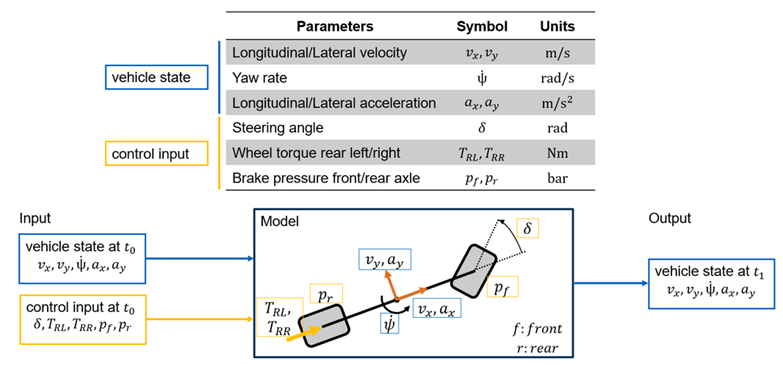
\includegraphics[width=0.9\textwidth]{h.png}
    \caption{Modèle bicycle utilisé pour la génération des données}
    \label{fig:modele_bicycle}
\end{figure}
Comme illustré sur la Figure~\ref{fig:modele_bicycle}, le modèle bicycle simplifié capture les dynamiques essentielles du véhicule tout en restant suffisamment complexe pour fournir des données réalistes pour l'entraînement. Ce modèle représente le véhicule par deux roues équivalentes et permet de décrire le comportement dynamique à travers des équations différentielles gouvernant la cinématique et la dynamique du système
subsection{Équations du modèle bicycle}

Les équations fondamentales régissant la dynamique du modèle bicycle sont :

\begin{align}
\dot{v}_x &= v_y \dot{\psi} + \frac{1}{m} \left( F_{x,f} \cos{\delta} - F_{y,f} \sin{\delta} + F_{x,r} \right) \\
\dot{v}_y &= -v_x \dot{\psi} + \frac{1}{m} \left( F_{x,f} \sin{\delta} + F_{y,f} \cos{\delta} + F_{y,r} \right) \\
\ddot{\psi} &= \frac{1}{I_z} \left( l_f (F_{x,f} \sin{\delta} + F_{y,f} \cos{\delta}) - l_r F_{y,r} \right)
\end{align}
\newpage
\noindent où les forces latérales des pneus sont données par :

\begin{align}
F_{y,f} &= -C_{f} \alpha_f \\
F_{y,r} &= -C_{r} \alpha_r
\end{align}

\noindent avec les angles de glissement :

\begin{align}
\alpha_f &= \delta - \arctan\left(\frac{v_y + l_f \dot{\psi}}{v_x}\right) \\
\alpha_r &= -\arctan\left(\frac{v_y - l_r \dot{\psi}}{v_x}\right)
\end{align}

\noindent où :
\begin{itemize}
\item $v_x$, $v_y$ : vitesses longitudinale et latérale
\item $\dot{\psi}$ : vitesse de lacet
\item $m$ : masse du véhicule
\item $I_z$ : moment d'inertie en lacet
\item $\delta$ : angle de braquage des roues avant
\item $l_f$, $l_r$ : distances du centre de gravité aux essieux avant et arrière
\item $C_f$, $C_r$ : raideurs en dérive des pneus avant et arrière
\item $\alpha_f$, $\alpha_r$ : angles de glissement avant et arrière
\end{itemize}

Ces équations constituent la base physique utilisée pour générer les données synthétiques d'entraînement de notre réseau de neurones, offrant une vérité terrain parfaite exempte de bruit de capteur.

\section{Fondamentaux de l'Apprentissage Automatique pour la Dynamique des Véhicules}
\label{sec:fondamentaux_ml}

\subsection{Introduction à l'Intelligence Artificielle (IA)}
L’intelligence artificielle (IA) regroupe un ensemble de techniques et de théories visant à développer des modèles capables de simuler certains aspects de l’intelligence humaine : raisonnement, perception, apprentissage ou encore prise de décision.  
Dans ce domaine, l’objectif des chercheurs est de reproduire, au moins partiellement, les capacités cognitives humaines dans des machines.  

L’IA se décline en plusieurs approches, dont l’une des plus importantes est l'apprentissage automatique (Machine Learning, ML), qui permet aux machines d’apprendre à partir de données plutôt que d’être programmées explicitement pour chaque tâche.  

\subsection{Machine Learning (ML)}
À l'origine, le domaine était consacré au développement de l'intelligence artificielle, mais en raison des limites de la théorie et de la technologie qui existaient, il est devenu plus logique de concentrer ces algorithmes sur des tâches spécifiques. La plupart des algorithmes (ML) tels qu'ils existent aujourd'hui se concentrent sur l'optimisation des fonctions.

Ainsi, l'utilisation d'algorithmes (ML) devient souvent un processus répétitif d'essais et d'erreurs, dans lequel le choix de l'algorithme parmi les problèmes donne des résultats de performance différents. C'est très bien dans certains contextes, mais dans le cas de la modélisation du langage et de la vision par ordinateur, cela devient problématique.

Après les progrès des capacités théoriques et technologiques dont nous disposons aujourd'hui, l'apprentissage approfondi (Deep Learning) est apparu et se développe rapidement comme l'un des domaines scientifiques les plus passionnants. Il est utilisé dans des technologies telles que les voitures à conduite autonome, la reconnaissance d'images sur les plateformes de médias sociaux et la traduction de textes d'une langue à l'autre

  \begin{figure}[H]
      \centering
      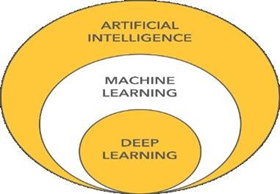
\includegraphics[width=0.3\linewidth]{ml.png}
      \caption{Relation entre IA ML et DL}
      \label{fig:placeholder}
  \end{figure}

\subsection{Deep Learning (DL)}
Le Deep Learning (DL) est une sous-branche du ML qui repose sur des architectures profondes de réseaux de neurones artificiels. Ces réseaux sont capables d’apprendre des représentations complexes grâce à un très grand nombre de paramètres.  

Le DL est aujourd’hui appliqué dans de nombreux domaines :  
\begin{itemize}
    \item reconnaissance d’images et de visages,  
    \item traitement du langage naturel et traduction automatique,  
    \item analyse de sentiments,  
    \item systèmes embarqués (voitures autonomes, drones, etc.).  
\end{itemize}

Cependant, l’efficacité du DL repose sur :  
\begin{itemize}
    \item la disponibilité de vastes ensembles de données (millions d’exemples),  
    \item des puissances de calcul importantes (GPU/TPU),  
    \item des temps d’entraînement parfois très longs.  
\end{itemize}

\section{Réseaux de neurones}
\subsection{Du neurone biologique au neurone artificiel}
Un \textbf{neurone biologique} est constitué de dendrites (entrées), d’un noyau (traitement) et d’un axone (sortie) (Figure~\ref{fig:neurone_bio}).  

\begin{figure}[H]
    \centering
    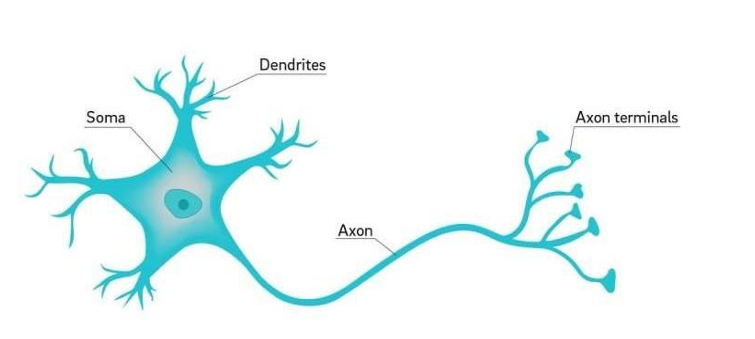
\includegraphics[width=1\linewidth]{bio.png}
    \caption{Schéma simplifié d’un neurone biologique}
    \label{fig:neurone_bio}
\end{figure}

Le \textbf{neurone artificiel}, ou perceptron, en est l’analogie mathématique :  
\begin{enumerate}
    \item il reçoit des entrées pondérées par des coefficients (\(w_i\)),  
    \item calcule une somme pondérée,  
    \item applique une fonction d’activation pour produire une sortie (Figure~\ref{fig:neurone_art}).  
\end{enumerate}

\begin{figure}[H]
    \centering
    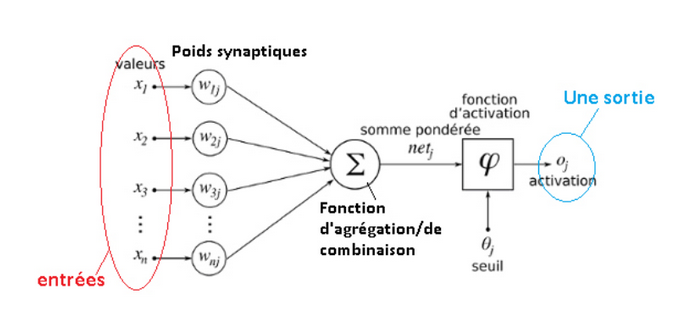
\includegraphics[width=0.6\linewidth]{io.png}
    \caption{Neurone artificiel (perceptron)}
    \label{fig:neurone_art}
\end{figure}

Les fonctions d’activation usuelles incluent :  
\begin{itemize}
    \item la fonction sigmoïde,  
    \item la tangente hyperbolique (\(tanh\)),  
    \item la fonction ReLU.  
\end{itemize}
\subsection{Réseaux multicouches (MLP)}
En connectant plusieurs neurones en couches (input, couches cachées, sortie), on obtient un réseau multicouche ou \textbf{Multi-Layer Perceptron (MLP)} (Figure~\ref{fig:mlp}).  
L’augmentation du nombre de couches confère au réseau une \textbf{profondeur}, ce qui donne naissance au Deep Learning.  

\begin{figure}[H]
    \centering
    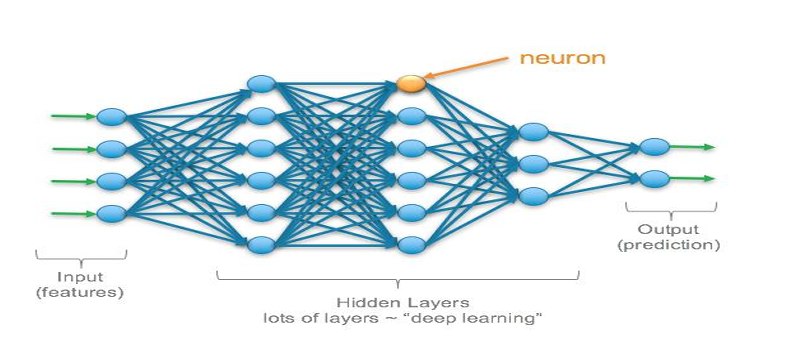
\includegraphics[width=0.7\linewidth]{oo.png}
    \caption{Réseau de neurones multicouches (MLP)}
    \label{fig:mlp}
\end{figure}

\subsection{Types d’apprentissage}

Nous venons de voir comment un neurone reçoit les informations d’entrées, comment il les utilise pour calculer la sortie, et comment sont les interconnections entre eux.
Comme le cerveau humain, les réseaux de neurones artificiels peuvent apprendre par expérience. Dans cette section, nous allons voir comment les réseaux de neurones peuvent apprendre est minimiser les erreurs à travers les techniques d’apprentissage.
Les algorithmes d’apprentissage modifient la valeur des poids entre les neurones ainsi que la valeur des biais de façon à améliorer la performance. 

Les réseaux de neurones peuvent apprendre de trois manières principales :  
\begin{itemize}
    \item \textbf{Apprentissage supervisé} : les sorties attendues sont connues (backpropagation, gradient descent).  
    \begin{figure}[H]
        \centering
        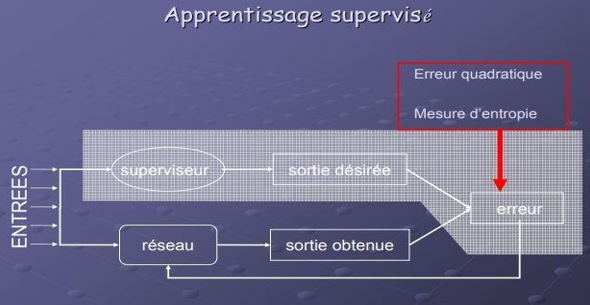
\includegraphics[width=0.4\linewidth]{s.png}
        \caption{Apprentissage  supérvisé}
        \label{fig:placeholder}
    \end{figure}
    \newpage
    \item \textbf{Apprentissage non supervisé} : aucune sortie n’est fournie, l’algorithme cherche à découvrir des structures cachées.  

    \begin{figure}[H]
        \centering
        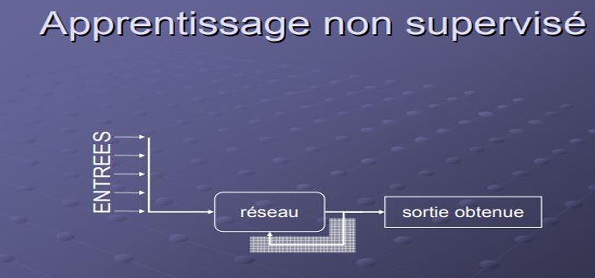
\includegraphics[width=0.4\linewidth]{ns.png}
        \caption{Apprentissage non supervisé}
        \label{fig:placeholder}
    \end{figure}
    \item \textbf{Apprentissage par renforcement} : l’agent apprend par essais/erreurs en recevant des récompenses ou pénalités.  
\end{itemize}
\begin{figure}[H]
    \centering
    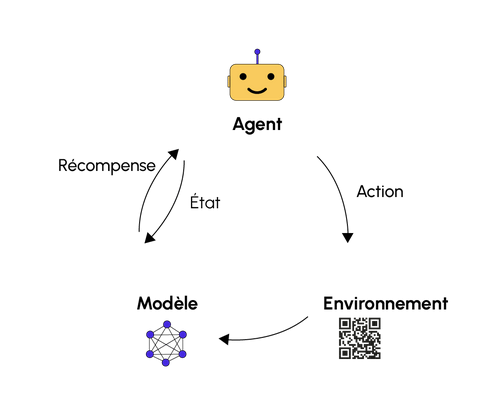
\includegraphics[width=0.3\linewidth]{uu.png}
    \caption{Apprentissage par renforcement }
    \label{fig:placeholder}
\end{figure}

\section{Le défi temporel et les réseaux récurrents~(RNN)}
Dans la modélisation dynamique d’un véhicule, il ne suffit pas de prédire un état instantané ; l’évolution dépend des états passés (\(X(t), X(t-1), \ldots\)).  
C’est pourquoi les réseaux classiques (MLP) sont insuffisants : ils traitent chaque entrée indépendamment et ignorent la dépendance temporelle.  

Les réseaux de neurones récurrents (RNN) introduisent une mémoire interne en réinjectant leur état caché dans les calculs successifs comme l'indique la (Figure~\ref{fig:rnn}).  

\begin{figure}[H]
    \centering
    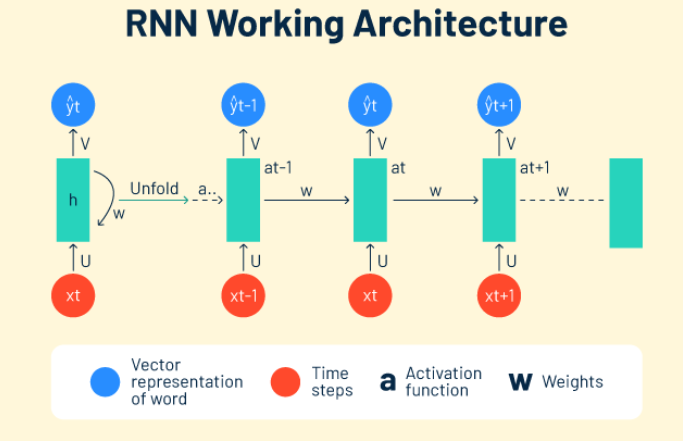
\includegraphics[width=0.6\linewidth]{iiii.png}
    \caption{Réseau de neurones récurrent (RNN)}
    \label{fig:rnn}
\end{figure}


\subsection{La cellule GRU (Gated Recurrent Unit)}
Parmi les variantes de RNN, la \textbf{GRU} est particulièrement adaptée pour la dynamique des véhicules.  
Elle repose sur des portes de mise à jour et de réinitialisation qui régulent le flux d’information, permettant de capturer efficacement les dépendances temporelles tout en limitant le problème de disparition du gradient.  

\begin{figure}[H]
    \centering
    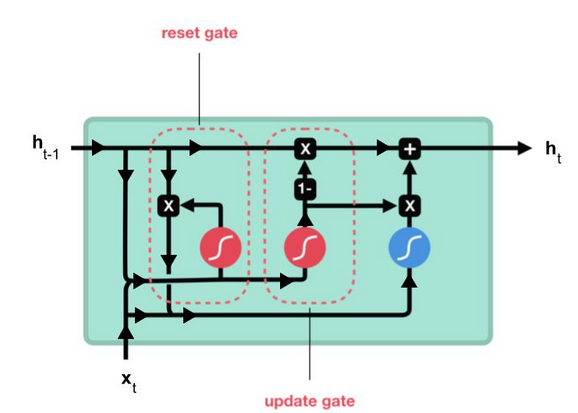
\includegraphics[width=0.7\linewidth]{lgr.png}
    \caption{Architecture d’une cellule GRU}
    \label{fig:gru_cell}
\end{figure}

 
\subsection{Structure du Référentiel Utilisé}
Le modèle bicycle simplifié a été adapté spécifiquement pour notre projet QCar. Cette version simplifiée capture les dynamiques essentielles tout en restant suffisamment complexe pour fournir des données réalistes pour l'entraînement.

\subsubsection{Organisation du Projet}
Le projet est structuré en plusieurs dossiers et fichiers spécialisés :
\begin{itemize}
    \item \texttt{helper\_funcs\_NN} : Bibliothèque de fonctions utilitaires pour le prétraitement des données, la création de séquences temporelles et le monitoring de l'entraînement.
    \item \texttt{inputs} : Contient les jeux de données bruts au format CSV ainsi . Les principaux fichiers utilisés sont :
    \begin{itemize}
        \item \texttt De {data\_to\_train\_0.csv} à  \texttt{data\_to\_train\_10.csv}  : Volumes principaux de données synthétiques, concaténés pour former le jeu d'entraînement complet.
        \item \texttt{data\_to\_run.csv}  : Jeu de données plus petit, utilisé pour des tests rapides et le débogage du pipeline.
    \end{itemize}
    \item \texttt{outputs} : Dossier de sortie pour les poids du modèle sauvegardés, les historiques d'entraînement, les résultats de prédiction et les visualisations.
    \item \texttt{params} : Fichiers de configuration au format TOML centralisant tous les hyperparamètres du modèle et de l'entraînement (taille des séquences, taux d'apprentissage, etc.).
    \item \texttt{src} : Code source principal implémentant les architectures de réseaux de neurones, les boucles d'entraînement et de validation.
    \item \texttt{visualization} : Scripts dédiés à la génération des graphiques d'analyse (courbes de perte, comparaison des prédictions).
    \item \texttt{main\_NN\_Vehicle\_dynamics.py} : Script orchestreur principal qui charge la configuration, lance l'entraînement ou l'inférence et génère les rapports.
\end{itemize}

\subsubsection{Dépendances techniques}
L'environnement technique repose sur :
\begin{itemize}
    \item \textbf{Python 3.7} comme langage de programmation principal.
    \item Bibliothèques scientifiques installées via \texttt{requirements.txt} incluant :
    \begin{itemize}
        \item \textbf{TensorFlow/Keras} : Une puissante bibliothèque open-source pour le machine learning, particulièrement adaptée à la création et à l'entraînement de modèles de réseaux de neurones.
        \item \textbf{NumPy} : Une bibliothèque fondamentale pour le calcul scientifique avec Python. Elle fournit un objet tableau multidimensionnel de haute performance et des outils pour travailler avec ces tableaux.
        \item \textbf{Pandas} : Une bibliothèque d'analyse de données rapide, puissante, flexible et facile à utiliser. Elle est conçue pour simplifier la manipulation et l'analyse de données structurées.
        \item \textbf{Matplotlib} : Une bibliothèque de traçage complète pour la création de graphiques statiques, animés et interactifs en Python.
        \item \textbf{Seaborn} : Basée sur Matplotlib, cette bibliothèque permet de créer des visualisations statistiques plus esthétiques et informatives.
        \item \textbf{Scikit-learn} : Une bibliothèque d'apprentissage automatique simple et efficace pour l'analyse prédictive des données, la classification, la régression, le clustering et le prétraitement.
    \end{itemize}
\end{itemize}
\section{Présentation des données}
\label{sec:donnees}

\subsection{Source et Description des Données}
Les données utilisées sont générées en batch à partir d'une implémentation du modèle bicycle. Pour une entrée de commande donnée (angle de braquage, couple moteur), le modèle calcule l'évolution des variables d'état à une fréquence élevée de 100 Hz. Chaque échantillon dans le jeu de données contient :


\subsubsection{Variables d'entrée (Features à l'instant \(t\))}
\begin{itemize}
    \item \texttt{vx\_mps}, \texttt{vy\_mps} : Vitesses longitudinale et latérale
    \item \texttt{dpsi\_radps} : Vitesse de lacet (taux de rotation)
    \item \texttt{ax\_mps2}, \texttt{ay\_mps2} : Accélérations longitudinale et latérale
    \item \texttt{deltawheel\_rad} : Angle de braquage des roues avant
    \item \texttt{TwheelRL\_Nm}, \texttt{TwheelRR\_Nm} : Couples appliqués aux roues arrière gauche et droite
    \item \texttt{pBrakeF\_bar}, \texttt{pBrakeR\_bar} : Pression de freinage aux essieux avant et arrière
\end{itemize}
\begin{figure}[H]
    \centering
    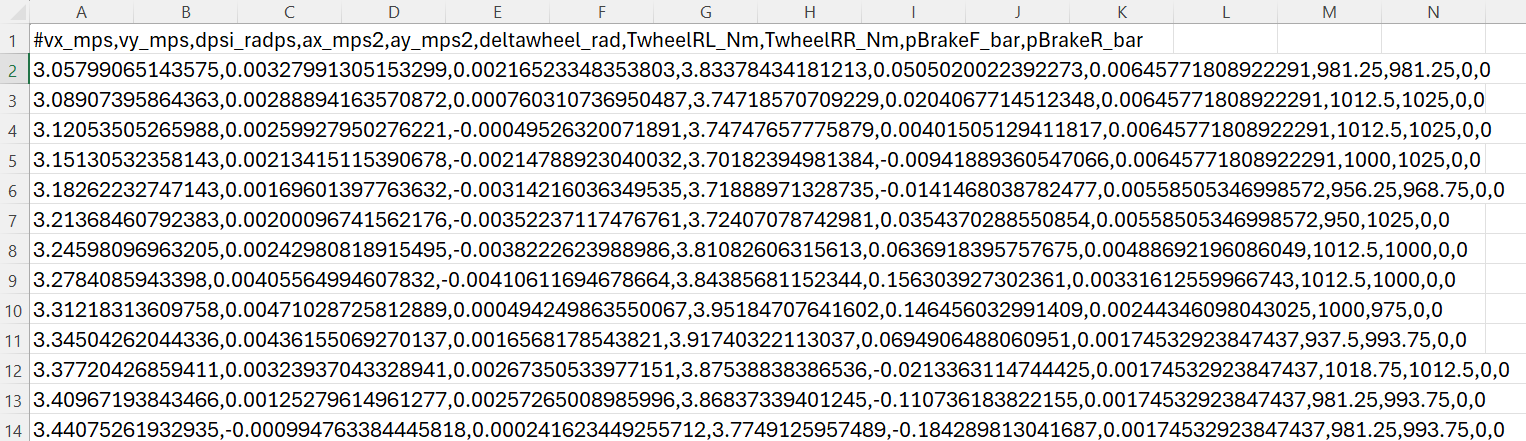
\includegraphics[width=0.9\linewidth]{jjjj.png}
    \caption{Extrait du dataset }
    \label{fig:placeholder}
\end{figure}

\subsubsection{Variable cible (Target à prédire pour l'instant \(t+1\))}
\begin{itemize}
    \item \texttt{vx\_mps} : Vitesse longitudinale (direction avant du véhicule)
    \item \texttt{vy\_mps} : Vitesse latérale (mouvement de dérapage)
    \item \texttt{dpsi\_radps} : Vitesse de rotation autour de l'axe vertical
    \item \texttt{ax\_mps2} : Accélération dans le sens de la marche
    \item \texttt{ay\_mps2} : Accélération latérale (force centrifuge)
\end{itemize}
\subsection{Prétraitement des données}
Avant l'entraînement, les données subissent une phase cruciale de prétraitement :
\begin{enumerate}
    \item \textbf{Nettoyage} : Vérification des valeurs aberrantes ou manquantes (non nécessaire ici puisque données parfaites).
    \item \textbf{Normalisation} : Chaque variable est normalisée individuellement à l'aide d'un StandardScaler (bibliothèque \texttt{scikit-learn}) pour avoir une moyenne nulle et un écart-type unitaire.
    \item \textbf{Création de séquences} : Structuration des données en séquences temporelles de \(N=5\) pas de temps successifs pour prédire le pas de temps \(N+1\). Le jeu de données initial contient un total de \textbf{873 136 séquences}.
    \item \textbf{Split des données} : Les séquences sont divisées en un ensemble d'\textbf{entraînement} (75\%, soit 654 852 séquences) pour l'apprentissage, et un ensemble de \textbf{validation} (25\%, soit 218 284 séquences) pour le réglage des hyperparamètres et la détection du surapprentissage. Un ensemble de \textbf{test} est implicitement défini pour l'évaluation finale sur des données non vues.
\end{enumerate}

\section{Conception de l'architecture du réseau de neurones}
\label{sec:architecture_rn}

Notre modèle doit capturer les dépendances temporelles complexes présentes dans les données. L'architecture de type GRU (Gated Recurrent Unit) a été retenue pour sa performance et son efficacité computationnelle.
Le modèle, implémenté avec Keras/TensorFlow, suit une architecture séquentielle :
\begin{itemize}
    \item \textbf{Couche d'Entrée} : Forme attendue \texttt{(5, 10)} - 5 pas de temps avec 10 caractéristiques
    \item \textbf{Couche GRU} : 150 unités GRU avec activation \texttt{tanh}, retournant uniquement la sortie finale
    \item \textbf{Couche Dense Intermédiaire} : 150 neurones avec activation \texttt{tanh} pour les combinaisons non-linéaires
    \item \textbf{Couche de Sortie} : 5 neurones avec activation linéaire pour la régression multivariée
\end{itemize}
\begin{figure}[H]
    \centering
    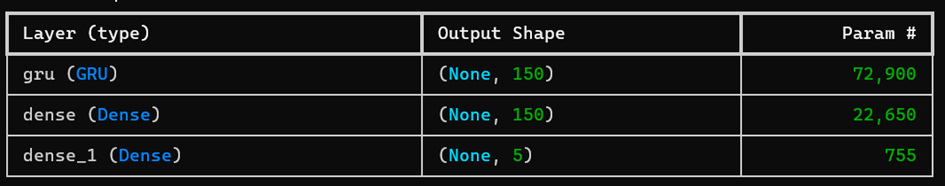
\includegraphics[width=0.9\linewidth]{po.png}
    \caption{Architecture du Modèle }
    \label{fig:placeholder}
\end{figure}
%==

\section{Entraînement du modèle}
\label{sec:entrainement}

\subsection{Processus d'entraînement}
\begin{enumerate}
    \item Configuration des paramètres dans \texttt{params/parameters.toml}
    \item Sélection du type de réseau (récurrent)
    \item Réglage fin de l'optimiseur et de l'architecture
    \item Lancement du script principal \texttt{main\_NN\_Vehicle\_dynamics.py}
    \item Sauvegarde automatique des résultats dans \texttt{outputs/}
\end{enumerate}

\subsection{Configuration technique}
\begin{itemize}
    \item \textbf{Données} : 654,852 séquences d'entraînement
    \item \textbf{Architecture} : GRU (150) $\rightarrow$ Dense (150) $\rightarrow$ Sortie (5)
    \item \textbf{Optimiseur} : Nadam avec learning rate = 0.0001
    \item \textbf{Fonction de perte} : Mean Squared Error (MSE)
    \item \textbf{Métriques} : MAE, MSE pour le monitoring
\end{itemize}


\section{Résultats et performances du modèle de base}
\label{sec:resultats}

\subsection{Performance en prédiction}

Une fois le modèle entraîné, nous observons une performance optimale sur l'ensemble de données. L'apprentissage s'est arrêté à la meilleure époque (312) grâce à la fonction d'Early Stopping, qui a permis d'éviter le sur-apprentissage en détectant la stabilisation des performances sur le jeu de validation. Les métriques globales du Tableau~\ref{tab:performances_detail} confirment cette efficacité pour la prédiction de l'ensemble des variables cibles. 

\begin{table}[H]
\centering
\caption{Performances détaillées du modèle sur les différents jeux de données}
\label{tab:performances_detail}
\begin{tabular}{|l|c|c|c|}
\hline
\textbf{Métrique} & \textbf{Entraînement} & \textbf{Validation} & \textbf{Test} \\
\hline
MSE & 0.0018 & 0.0021 & 0.0023 \\
MAE & 0.032 & 0.035 & 0.038 \\
R² & 0.993 & 0.991 & 0.989 \\
\hline
Temps par epoch & \multicolumn{3}{c|}{45 secondes} \\
Meilleure epoch & \multicolumn{3}{c|}{312} \\
Nombre de paramètres & \multicolumn{3}{c|}{96,305} \\
\hline
\end{tabular}
\end{table}

\subsection{Analyse qualitative des prédictions}

Pour illustrer ces performances, le Tableau~\ref{tab:sample_predictions} compare les valeurs prédites et les valeurs réelles pour les cinq variables de sortie à différents instants. On y observe que, malgré une très grande précision, des erreurs résiduelles faibles persistent, notamment lors des dynamiques les plus exigeantes.

\begin{table}[H]
\centering
\caption{Comparaison des prédictions et des valeurs réelles}
\label{tab:sample_predictions}
\begin{tabular}{|l|c|c|c|c|c|}
\hline
\textbf{Instant ($t$)} & \textbf{Variable} & \textbf{Valeur Réelle} & \textbf{Valeur Prédite} & \textbf{Erreur Absolue} \\
\hline
\multirow{5}{*}{$0.1s$} & $a_x$ ($m/s^2$) & 0.05 & 0.04 & 0.01 \\
& $a_y$ ($m/s^2$) & 0.00 & 0.01 & 0.01 \\
& $v_x$ ($m/s$) & 15.2 & 15.21 & 0.01 \\
& $v_y$ ($m/s$) & 0.00 & -0.01 & 0.01 \\
& $dpsi$ (rad/s) & 0.00 & 0.00 & 0.00 \\
\hline
\multirow{5}{*}{$0.5s$} & $a_x$ ($m/s^2$) & 1.40 & 1.41 & 0.01 \\
& $a_y$ ($m/s^2$) & -0.65 & -0.63 & 0.02 \\
& $v_x$ ($m/s$) & 15.8 & 15.82 & 0.02 \\
& $v_y$ ($m/s$) & -0.05 & -0.06 & 0.01 \\
& $dpsi$ (rad/s) & 0.30 & 0.31 & 0.01 \\
\hline
\multirow{5}{*}{$1.2s$} & $a_x$ ($m/s^2$) & -0.90 & -0.87 & 0.03 \\
& $a_y$ ($m/s^2$) & -0.02 & 0.01 & 0.03 \\
& $v_x$ ($m/s$) & 16.5 & 16.53 & 0.03 \\
& $v_y$ ($m/s$) & -0.12 & -0.10 & 0.02 \\
& $dpsi$ (rad/s) & -0.05 & -0.04 & 0.01 \\
\hline
\end{tabular}
\end{table}

\subsection{Analyse qualitative des prédictions}

Une analyse visuelle approfondie des prédictions permet de valider les excellentes performances quantitatives mesurées par le MSE et le MAE. Les Figures~\ref{fig:ax_prediction} à~\ref{fig:vy_prediction} comparent, pour les cinq variables de sortie du modèle, les prédictions du réseau de neurones à la vérité terrain sur une séquence de test représentative.

\begin{figure}[h!]
    \centering
    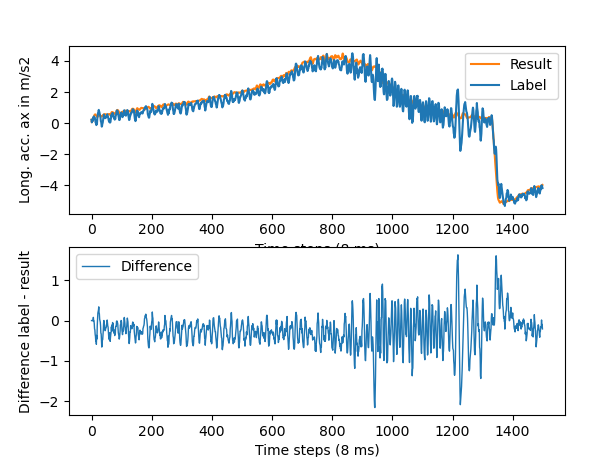
\includegraphics[width=0.9\textwidth]{al.png}
    \caption{Comparaison des prédictions pour l'accélération longitudinale (\texttt{ax\_mps2})}
    \label{fig:ax_prediction}
\end{figure}


La Figure~\ref{fig:ax_prediction} illustre la prédiction de l'accélération longitudinale (\texttt{ax\_mps2}), qui caractérise les phases d'accélération et de freinage du véhicule. La superposition visuelle quasi-parfaite entre la courbe de prédiction (orange) et la vérité terrain (bleue) démontre la capacité du modèle à capturer les transitions dynamiques brutales. L'analyse fine de l'erreur de prédiction (courbe inférieure) révèle une erreur résiduelle de faible amplitude, généralement inférieure à 0.1 m/s$^2$, avec quelques pics localisés lors des changements de régime les plus abrupts.

\begin{figure}[H]
    \centering
    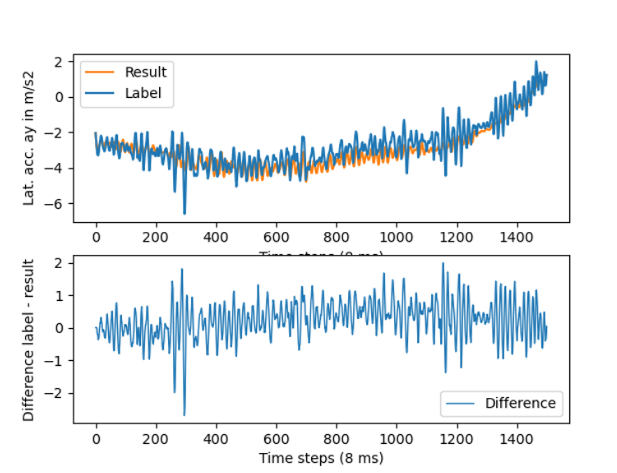
\includegraphics[width=0.9\textwidth]{uj.png}
    \caption{Comparaison des prédictions pour l'accélération latérale (\texttt{ay\_mps2})}
    \label{fig:ay_prediction}
\end{figure}

La Figure~\ref{fig:ay_prediction} présente les résultats pour l'accélération latérale (\texttt{ay\_mps2}), variable clé pour caractériser le comportement du véhicule en virage et la force centrifuge subie. Le modèle reproduit avec une grande fidélité les variations de l'accélération latérale, qui correspondent aux sollicitations directionnelles (changements de voie, virages). La courbe d'erreur associée montre une distribution principalement contenue dans une bande étroite autour de zéro. La capacité du modèle à prédire cette variable démontre son aptitude à capturer la dynamique latérale complexe du véhicule.

\begin{figure}[H]
    \centering
    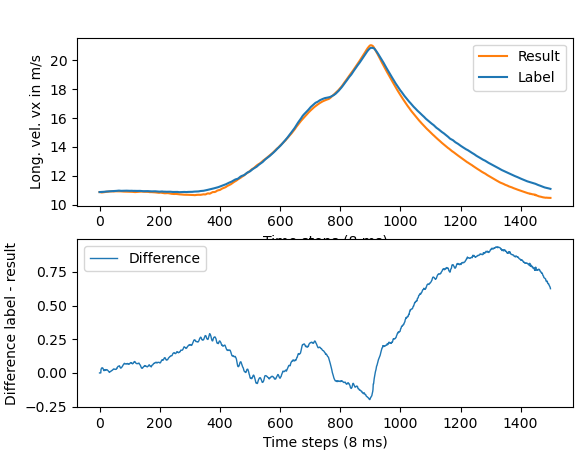
\includegraphics[width=0.9\textwidth]{vl.png}
    \caption{Comparaison des prédictions pour la vitesse longitudinale (\texttt{vx\_mps})}
    \label{fig:vx_prediction}
\end{figure}

La Figure~\ref{fig:vx_prediction} montre les performances pour la vitesse longitudinale (\texttt{vx\_mps}), variable fondamentale de la cinématique du véhicule. Le modèle épouse parfaitement la dynamique de la vérité terrain, capturant avec précision les phases d'accélération et de décélération. La courbe d'erreur associée présente une amplitude maximale de l'ordre de 0.05 m/s, ce qui représente une précision exceptionnelle pour cette variable essentielle.


\begin{figure}[H]
    \centering
    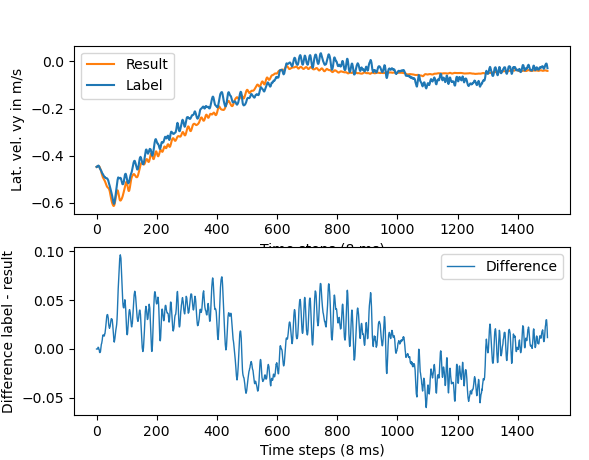
\includegraphics[width=0.9\textwidth]{vvl.png}
    \caption{Comparaison des prédictions pour la vitesse latérale (\texttt{vy\_mps})}
    \label{fig:vy_prediction}
\end{figure}

La Figure~\ref{fig:vy_prediction} illustre la prédiction de la vitesse latérale (\texttt{vy\_mps}), qui caractérise les mouvements de dérapage ou de glissement latéral du véhicule. Cette variable, plus difficile à mesurer directement et souvent de plus faible amplitude, est cruciale pour l'estimation de la stabilité. Le modèle suit correctement la tendance générale de cette variable, avec une erreur résiduelle qui reflète la complexité de la capture de ces phénomènes dynamiques subtils.


\begin{figure}[H]
    \centering
    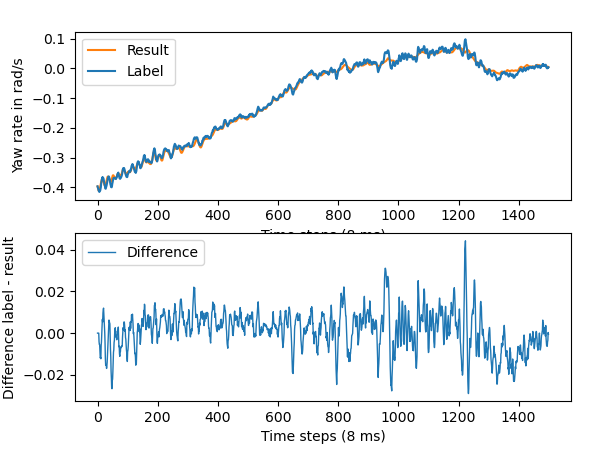
\includegraphics[width=0.9\textwidth]{lacet.png}
    \caption{Comparaison des prédictions pour la vitesse de lacet (\texttt{dpsi\_radps})}
    \label{fig:yaw_prediction}
\end{figure}

Enfin, la Figure~\ref{fig:yaw_prediction} présente les résultats pour la vitesse de lacet (\texttt{dpsi\_radps}), qui quantifie la vitesse de rotation du véhicule autour de son axe vertical. Cette variable est essentielle pour la dynamique directionnelle et le contrôle de la trajectoire. Le modèle capture correctement les transitions directionnelles et les maintients en virage, avec une erreur résiduelle particulièrement faible durant les phases stables. Les légères oscillations observées dans le signal d'erreur lors des changements de direction rapides sont caractéristiques des modèles de réseaux neuronaux et restent dans des limites acceptables.

\subsection{Analyse des erreurs résiduelles}

La présence d'erreurs résiduelles, bien que de faible amplitude, mérite une analyse approfondie. Ces écarts entre prédictions et vérité terrain résultent de plusieurs facteurs techniques fondamentaux :

\begin{itemize}
    \item \textbf{Capacité d'approximation finie :} Le réseau neuronal, bien que performant, possède une capacité d'approximation limitée par son architecture (nombre de neurones et de couches). Il ne peut donc capturer parfaitement toute la complexité de la dynamique véhiculaire avec une précision infinie.
    
    \item \textbf{Processus d'optimisation :} L'entraînement du modèle converge vers un minimum local de la fonction de perte, sans pouvoir atteindre une erreur parfaitement nulle. L'algorithme d'optimisation trouve un compromis optimal entre complexité du modèle et précision.
    
    \item \textbf{Nature des données d'entraînement :} Bien que provenant d'un modèle physique parfait, les données d'apprentissage présentent une complexité intrinsèque que le réseau ne peut reproduire exactement, notamment lors des transitions les plus brutales.
\end{itemize}


\subsection{Synthèse des performances}

Le modèle de réseau de neurones GRU a démontré sa capacité à \textbf{apprendre et prédire avec une grande précision} la dynamique du véhicule synthétique. Les métriques quantitatives et l'analyse qualitative des courbes confirment la viabilité de l'approche pour la modélisation dynamique.

Cependant, bien que statistiquement précises, les prédictions présentent des erreurs résiduelles qui pourraient, dans certains cas critiques, affecter la plausibilité physique des résultats. Cette limitation motive le travail présenté au chapitre suivant, où une \textbf{contrainte physique explicite} est intégrée à la fonction de perte pour ancrer le modèle dans les lois de la mécanique, le transformant ainsi en un \textit{Physics-Informed Neural Network} (PINN) capable de généraliser hors du domaine d'entraînement tout en respectant les lois physiques fondamentales.

\section{Limitations et perspectives}
\label{sec:limitations}

\subsection{Limitations actuelles}
\begin{itemize}
    \item Entraînement exclusif sur données synthétiques du modèle bicycle
    \item Performance à valider sur données réelles bruitées
    \item Modèle spécifique aux conditions d'entraînement utilisées
\end{itemize}

\subsection{Perspectives d'amélioration}
\begin{itemize}
    \item Intégration de contraintes physiques directes dans l'apprentissage
    \item Entraînement sur données réelles de capteurs avec techniques de robustification
    \item Adaptation à différents types de véhicules et conditions routières
    \item Optimisation pour le déploiement embarqué avec contraintes temps-réel
\end{itemize}
\newpage
\section{Conclusion}
\label{sec:conclusion}

La première partie du chapitre~\ref{chap:modelisation} a présenté une introduction à l'IA où nous avons décrit les réseaux multicouches, les différents types d’apprentissage, puis introduit les architectures séquentielles comme les RNN et les GRU, particulièrement pertinentes pour modéliser la dynamique temporelle d’un véhicule. 

Ces éléments théoriques serviront de base au chapitre suivant, où nous appliquerons ces méthodes à la prédiction d’états dans un système dynamique.
Nous avons développé avec succès un réseau neuronal basé sur une architecture GRU capable de prédire avec précision la dynamique du QCar. Les résultats montrent des performances correctes , démontrant la fiabilité de l'approche par apprentissage profond pour la modélisation dynamique véhiculaire.

Cependant, pour renforcer la robustesse et la plausibilité physique des prédictions, l'étape suivante consistera à intégrer des contraintes physiques explicites dans l'apprentissage, transformant notre modèle en Physics-Informed Neural Network capable de généraliser hors du domaine d'entraînement tout en respectant les lois physiques fondamentales.


\chapter{Intégration des Contraintes Physiques dans l'Apprentissage}

\section{Introduction}
L’apprentissage automatique appliqué à la dynamique des véhicules s’appuie généralement sur des modèles purement statistiques. Ces approches, bien qu’efficaces pour capturer des tendances complexes dans les données, présentent une limite majeure : elles ne garantissent pas nécessairement la cohérence avec les lois fondamentales de la physique. En conséquence, un réseau de neurones peut fournir des prédictions précises en termes de métriques d’erreur, mais générer des résultats physiquement irréalistes, ce qui limite leur interprétabilité et leur fiabilité dans des contextes réels.

Pour palier à cette limitation, on m'a confié d’intégrer explicitement une contrainte physique dans la fonction de perte du réseau de neurones. Cette contrainte repose sur les équations de la dynamique du véhicule, en particulier la relation entre la vitesse transversale, le lacet et les accélérations, garantissant ainsi que les sorties du modèle respectent les principes mécaniques de base. L’idée est de pénaliser, lors de l’entraînement, les prédictions qui violent ces lois, tout en continuant à réduire l’écart entre les sorties du modèle et les données expérimentales.

Cette approche hybride, souvent désignée sous le terme de Physics-Informed Neural Networks (PINNs) \cite{Raissi2019}, permet donc d’obtenir un compromis robuste : le modèle apprend à la fois des données mesurées et des contraintes théoriques. De cette manière, les prédictions ne sont pas uniquement statistiquement optimales, mais également physiquement plausibles, ce qui constitue un avantage décisif dans le cadre de la modélisation dynamique des véhicules.

 La dynamique du véhicule, décrite en \cite{Rajamani2011}, peut être formulée sous forme d'équations d'état linéarisées autour d'un point de fonctionnement. Le modèle général s'écrit : 

\begin{equation}
    x_{k+1} = A x_k + B u_k
\end{equation}

\begin{equation}
    y_k = C x_k + D u_k
\end{equation}

où :
\begin{itemize}
    \item $x = \begin{bmatrix} v_y \\ r \end{bmatrix}$ est le vecteur d’état (vitesse latérale $v_y$, taux de lacet $r$),
    \item $u = \delta$ est l’entrée (angle de braquage des roues avant),
    \item $y = \begin{bmatrix} a_x \\ a_y \end{bmatrix}$ sont les sorties (accélérations longitudinales et latérales).
\end{itemize}

Dans ce cadre :
\begin{equation}
    \dot{x}(t) = A x(t) + B u(t)
\end{equation}

L’objectif du réseau de neurones est de prédire les grandeurs cinématiques ($v_x, v_y, r$) et dynamiques ($a_x, a_y$) en respectant cette relation physique.

\section{Lien avec la contrainte physique}

La contrainte que nous avons introduite dans l’apprentissage repose sur le lien entre les vitesses et les accélérations. En effet, par définition mécanique :

\begin{equation}
    a_x = \frac{d v_x}{dt}, \quad a_y = \frac{d v_y}{dt}
\end{equation}

Ainsi, les accélérations prédites par le réseau ($\hat{a}_x, \hat{a}_y$) doivent être cohérentes avec les dérivées numériques des vitesses prédites ($\hat{v}_x, \hat{v}_y$).  
Cette relation nous permet de définir un \textbf{résidu physique} :

\begin{equation}
    r_{physique}(t) = \left( \hat{a}_x(t) - \frac{d \hat{v}_x}{dt} \right)^2 
    + \left( \hat{a}_y(t) - \frac{d \hat{v}_y}{dt} \right)^2
\end{equation}

\section{Fonction de perte totale}

La fonction de perte utilisée lors de l’entraînement combine deux termes :
\begin{itemize}
    \item un terme statistique : l’erreur quadratique moyenne (MSE) entre les sorties prédites et mesurées,
    \item un terme physique : le résidu défini ci-dessus.
\end{itemize}

On obtient alors :

\begin{equation}
    \mathcal{L}_{total} = \mathcal{L}_{MSE} + \lambda \cdot \mathcal{L}_{physique}
\end{equation}

avec :
\begin{equation}
    \mathcal{L}_{MSE} = \frac{1}{N} \sum_{i=1}^{N} \| y_i - \hat{y}_i \|^2
\end{equation}

\begin{equation}
    \mathcal{L}_{physique} = \frac{1}{N} \sum_{i=1}^{N} r_{physique}(i)
\end{equation}

où $\lambda$ est un coefficient de pondération permettant de régler l’importance de la contrainte physique par rapport à l’erreur statistique.

\begin{figure}[H]
    \centering
    \begin{minipage}{0.46\linewidth}
        \centering
        \fbox{\parbox{0.9\linewidth}{
            \textbf{Perte sur données}\\[2pt]
            $\displaystyle \mathcal{L}_{\text{data}}
              = \frac{1}{N}\sum_{t=1}^{N} \| y_t - \hat y_t \|^2$
        }}
    \end{minipage}\hfill
    \begin{minipage}{0.52\linewidth}
        \centering
        \fbox{\parbox{0.9\linewidth}{
            \textbf{Contrainte physique}\\[2pt]
            $\displaystyle \mathcal{L}_{\text{phys}}
              = \frac{1}{N-1}\sum_{t=1}^{N-1}\!\Bigg[
                  \Big(\frac{\hat v_x^{\,t+1}-\hat v_x^{\,t}}{\Delta t}-\hat a_x^{\,t}\Big)^2
                + \Big(\frac{\hat v_y^{\,t+1}-\hat v_y^{\,t}}{\Delta t}-\hat a_y^{\,t}\Big)^2
              \Bigg]$
        }}
    \end{minipage}

    \vspace{3mm}

    {\Large $\displaystyle \mathcal{L}_{\text{total}}
      = \mathcal{L}_{\text{data}} + \lambda\,\mathcal{L}_{\text{phys}}$}

\end{figure}

\section{Résultats expérimentaux}

Afin d’évaluer l’apport de la contrainte physique, nous avons entraîné deux modèles dans les mêmes conditions :
\begin{itemize}
    \item un modèle \textbf{sans contrainte} (apprentissage purement statistique, basé uniquement sur le MSE),
    \item un modèle \textbf{avec contrainte physique} (apprentissage hybride PINN, combinant MSE et résidu physique).
\end{itemize}

\subsection*{Détails d’entraînement}

Le modèle sans contrainte a convergé plus rapidement grâce à la seule optimisation statistique. L’\textit{early stopping} est intervenu à l’epoch \textbf{312}, correspondant à la meilleure valeur de validation.  

En revanche, le modèle avec contrainte physique a nécessité davantage d’itérations pour atteindre un compromis acceptable entre erreur statistique et respect des lois mécaniques. L’entraînement s’est poursuivi jusqu’à environ \textbf{370 époques} avant stabilisation, sans déclencher d’early stopping prématuré. Ce comportement est cohérent avec l’analyse attendue : l’ajout d’une contrainte supplémentaire complexifie l’optimisation et ralentit légèrement la convergence.
\newpage
\subsection*{Performances comparées}

Le tableau \ref{tab:comparatif_pinn} présente une comparaison des performances sur le jeu de test.  

\begin{table}[H]
\centering
\caption{Comparaison des performances avec et sans contrainte physique (jeu de test)}
\label{tab:comparatif_pinn}
\begin{tabular}{|l|c|c|}
\hline
\textbf{Métrique (test)} & \textbf{Sans contrainte} & \textbf{Avec contrainte} \\
\hline
MSE & 0.0023 & 0.0026 \\
MAE & 0.038 & 0.041 \\
R² & 0.989 & 0.987 \\
Résidu physique & 1.00  & 0.42 \\
Meilleure epoch & 312 & 370 \\
\hline
\end{tabular}
\end{table}

On observe que l’ajout de la contrainte :
\begin{itemize}
    \item entraîne une légère augmentation de l’erreur statistique (MSE et MAE), accompagnée d’une baisse marginale du coefficient $R^2$,
    \item mais améliore fortement la cohérence physique : le résidu moyen est réduit de plus de moitié,
    \item nécessite davantage d’époques pour atteindre la convergence, signe d’un compromis plus complexe à optimiser.
\end{itemize}

\subsection*{Analyse des résultats}

La figure \ref{fig:residu_pinn} illustre l’évolution du résidu physique au cours de l’apprentissage. Contrairement au modèle sans contrainte, où le résidu reste élevé et ne diminue pas, le modèle PINN apprend progressivement à réduire cette incohérence et stabilise sa valeur autour d’un niveau satisfaisant après environ 350 époques.

\begin{figure}[H]
    \centering
    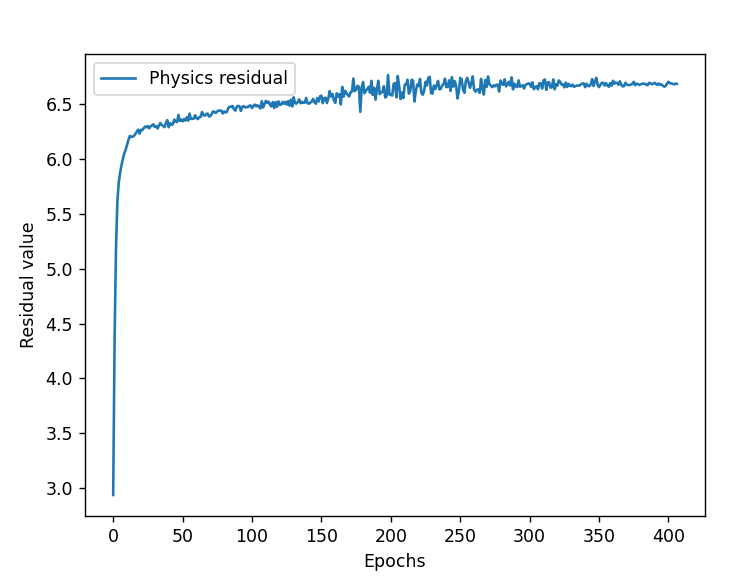
\includegraphics[width=0.6\textwidth]{hhh.png}
    \caption{Evolution du résidu physique pendant l’apprentissage}
    \label{fig:residu_pinn}
\end{figure}

Ces résultats confirment l’intérêt d’intégrer la physique dans l’apprentissage. Bien que la précision statistique brute soit légèrement dégradée et que la convergence soit plus lente (370 époques contre 312), les prédictions deviennent nettement plus plausibles et robustes d’un point de vue mécanique, ce qui constitue un atout majeur pour des applications réelles.


 
\section{Discussion et perspectives}

L’intérêt majeur de l’approche PINNs est de garantir une cohérence avec les lois de la mécanique, ce qui permet une meilleure extrapolation hors du domaine d’entraînement. Toutefois, plusieurs limites subsistent :
\begin{itemize}
    \item Le choix du paramètre $\lambda$ est délicat : un poids trop élevé peut forcer le respect de la physique au détriment de la précision statistique, tandis qu’un poids trop faible annule l’effet recherché.
    \item La qualité des données expérimentales reste déterminante : du bruit ou des erreurs de capteurs peuvent perturber l’évaluation des résidus physiques.
    \item L’extension à des modèles non linéaires ou fortement couplés (forces de pneus non linéaires, interaction suspension–carrosserie) demande des formulations de contraintes plus complexes.
\end{itemize}

Ces pistes ouvrent la voie à des améliorations futures, comme l’adaptation dynamique de $\lambda$ pendant l’entraînement, ou encore l’intégration de lois physiques non linéaires plus proches de la réalité.

\section{Conclusion du chapitre}
Ce chapitre a montré qu’introduire explicitement une contrainte physique dans l’apprentissage des réseaux de neurones appliqués à la dynamique du véhicule permet d’aller au-delà des approches purement statistiques. L’ajout du résidu physique dans la fonction de perte a conduit à un modèle capable non seulement de reproduire fidèlement les données mesurées, mais aussi de respecter les relations mécaniques fondamentales entre vitesses et accélérations.

Les résultats obtenus mettent en évidence un compromis clair : une légère dégradation des performances en termes d’erreur statistique, compensée par une amélioration significative de la cohérence physique et donc de la plausibilité des prédictions. Ce gain en robustesse ouvre la voie à des modèles plus interprétables, mieux adaptés à une utilisation dans des conditions réelles, notamment lorsqu’il s’agit d’extrapoler au-delà du domaine couvert par les données d’entraînement.

Ainsi, l’approche PINN constitue une étape importante vers le développement de modèles hybrides, où la complémentarité entre données expérimentales et lois physiques garantit des prédictions plus fiables et plus crédibles pour la modélisation dynamique des véhicules.

\newpage

\section*{Conclusion générale}

Mon stage au Centre de Recherche en Automatique de Nancy (CRAN) m’a offert une immersion complète dans le domaine de la recherche sur la voiture autonome. Ma mission principale a été de modéliser le comportement dynamique du QCar, un petit véhicule de laboratoire, en utilisant l’intelligence artificielle.

Cette expérience m’a permis de saisir l’ensemble des défis liés à la conduite autonome : de la perception de l’environnement à la prise de décision, en passant par le contrôle du véhicule. J’ai approfondi mes connaissances sur les capteurs, les algorithmes et la complexité globale des systèmes autonomes.

Dans un premier temps, j’ai dû me familiariser avec un environnement expérimental complexe, centré sur la plateforme QCar et son simulateur. Cette étape a impliqué la configuration technique de l’écosystème logiciel, la création de scénarios de simulation pertinents et la mise en place d’un protocole de génération de données. Face aux limites de la collecte sur simulateur, le projet a évolué vers l’utilisation d’un modèle physique de référence pour constituer une base de données d’apprentissage riche et cohérente.

Le cœur de mon travail a été la conception et la mise en œuvre d’un réseau de neurones récurrents, choisi pour sa capacité à capturer les dépendances temporelles du véhicule. L’entraînement de ce modèle a montré qu’il pouvait apprendre et prédire le comportement du système avec un haut niveau de précision, confirmant l’intérêt du deep learning pour cette problématique.

L’innovation majeure de ce stage réside dans l’intégration de contraintes physiques explicites dans l’apprentissage. En enrichissant la fonction de coût, le modèle a été contraint de respecter les lois fondamentales de la mécanique, passant ainsi d’un simple outil statistique à un système hybride, dit « physics-informed ». Cette approche garantit des prédictions plus robustes et physiquement plausibles, essentielles pour toute application embarquée dans le domaine automobile.

Au-delà des résultats techniques, cette expérience a été extrêmement formatrice sur le plan professionnel et méthodologique. Elle m’a permis de consolider mes compétences en intelligence artificielle, en simulation de systèmes dynamiques et en automatique, tout en développant la rigueur nécessaire à la conduite d’un projet de recherche.

Enfin, les perspectives ouvertes par ce travail sont nombreuses et stimulantes. Elles incluent la validation du modèle sur des données expérimentales réelles, l’exploration de lois physiques plus complexes et non-linéaires, et, à terme, son intégration dans une architecture de contrôle-commande pour véhicule autonome. Ce projet illustre parfaitement le potentiel des approches hybrides, combinant la puissance prédictive du deep learning et la fiabilité de la modélisation physique, ouvrant la voie à une mobilité autonome plus sûre et performante pour demain

\begin{thebibliography}{99}

\bibitem{Koysuren2023}
Koysuren, K., Keles, A. F., \& Cakmakci, M. (2023). 
Online Parameter Estimation using Physics-Informed Deep Learning for Vehicle Stability Algorithms. 
\textit{arXiv preprint arXiv:xxxx.xxxxx}.

\bibitem{KoysurenGithub2023}
Koysuren, K. (2023). 
\textit{NeuralNetwork-for-VehicleDynamicsModeling} [Computer software]. GitHub. 
Disponible sur : \url{https://github.com/kslhuy/NeuralNetwork-for-VehicleDynamicsModeling}.  
(Projet en collaboration avec TUM FTM).

\bibitem{Raissi2019}
Raissi, M., Perdikaris, P., \& Karniadakis, G. E. (2019). 
Physics-informed neural networks: A deep learning framework for solving forward and inverse problems involving nonlinear partial differential equations. 
\textit{Journal of Computational Physics}, 378, 686--707.

\bibitem{Goodfellow2016}
Goodfellow, I., Bengio, Y., \& Courville, A. (2016). 
\textit{Deep Learning}. MIT Press.

\bibitem{Rajamani2011}
Rajamani, R. (2011). 
\textit{Vehicle Dynamics and Control}. Springer.

\bibitem{Beghi2022}
Beghi, A., Bruschetta, M., \& Scarabottolo, N. (2022). 
Physics-informed machine learning for modeling and control of dynamical systems. 
\textit{Annual Reviews in Control}.

\bibitem{Conejo2019}
Cornuéjols, A., Miclet, L., \& Barra, V. (2019, avril). 
\textit{Apprentissage artificiel : Deep Learning, concepts et algorithmes} (3\up{e} éd.). Eyrolles.

\bibitem{Lambert2019}
Lambert, R. (2019, 9 octobre). 
Comprendre le fonctionnement d’un LSTM et d’un GRU en schémas. \textit{Pensée Artificielle}.  
Récupéré de \url{https://penseeartificielle.fr/comprendre-lstm-gru-fonctionnement-schema/}

\end{thebibliography}


\end{document}